\documentclass[12pt,a4paper]{article}

\usepackage[utf8]{inputenc}
\usepackage[T5]{fontenc}
\usepackage[vietnamese]{babel}
\usepackage{geometry}
\usepackage{setspace}
\usepackage{graphicx}
\usepackage{array}
\usepackage{longtable}
\usepackage{booktabs}
\usepackage{tabularx}
\usepackage{enumitem}
\usepackage{hyperref}
\usepackage{xcolor}
\usepackage{fancyhdr}
\usepackage{titlesec}
\usepackage{indentfirst}
\usepackage{amsmath}
\usepackage{float}

\geometry{margin=2.5cm}
\graphicspath{{imgs/}}
\onehalfspacing
\setlength{\parskip}{0.25em}

\hypersetup{
    colorlinks=true,
    linkcolor=blue!60!black,
    urlcolor=blue!60!black
}

\newcommand{\LogoPath}{logo-truong.png}

\pagestyle{fancy}
\fancyhf{}
\lhead{%
    \IfFileExists{\LogoPath}{%
        \raisebox{-0.25\height}{\includegraphics[height=0.8cm]{\LogoPath}}\hspace{0.5em}%
    }{}%
    \small Báo cáo hệ thống quản lý thư viện%
}
\rhead{Trang \thepage}
\renewcommand{\headrulewidth}{0.4pt}
\setlength{\headheight}{24pt}

\titleformat{\section}{\large\bfseries}{\thesection.}{0.6em}{}
\titleformat{\subsection}{\normalsize\bfseries}{\thesubsection.}{0.6em}{}
\titleformat{\subsubsection}{\normalsize\bfseries}{\thesubsubsection.}{0.6em}{}

\newcommand{\UniversityName}{TRƯỜNG ĐẠI HỌC THỦ ĐÔ HÀ NỘI}
\newcommand{\FacultyName}{KHOA CÔNG NGHỆ THÔNG TIN}
\newcommand{\ReportTitle}{BÁO CÁO DỰ ÁN NHÓM}
\newcommand{\ProjectCourse}{TIẾNG ANH CHUYÊN NGÀNH}
\newcommand{\ProjectName}{HỆ THỐNG QUẢN LÝ THƯ VIỆN}
\newcommand{\GroupNumber}{38}
\newcommand{\DepartmentName}{Công nghệ thông tin}
\newcommand{\AcademicYear}{2025--2026}

\begin{document}

% ===================== TRANG BÌA =====================
\begin{titlepage}
\centering
\vspace*{0.8cm}

{\Large \textbf{\UniversityName}}\\[0.3cm]
{\large \textbf{\FacultyName}}\\[0.9cm]

\IfFileExists{\LogoPath}{
    \includegraphics[width=0.32\textwidth]{\LogoPath}\\[0.45cm]
}{
    \fbox{
        \begin{minipage}[c][3.6cm][c]{5.2cm}
            \centering
            \textbf{LOGO TRƯỜNG}\\
            (thay \texttt{logo-truong.png})
        \end{minipage}
    }\\[0.45cm]
}

\rule{\textwidth}{0.8pt}\\[0.45cm]
{\LARGE \textbf{\ReportTitle}}\\[0.25cm]
\rule{\textwidth}{0.8pt}\\[0.95cm]

{\Large \textbf{\ProjectCourse}}\\[0.2cm]
{\LARGE \textbf{\ProjectName}}\\[0.85cm]

{\large \textbf{Danh sách thành viên}}\\[0.25cm]
\begin{tabular}{rl}
Hoang Kim Long & 223001755 \\
Nguyen Ngoc Tuan & 223001807 \\
Pham Gia Bao & 223001696 \\
\end{tabular}

\vspace{0.55cm}
\begin{center}
\begin{tabular}{p{4cm} p{8cm}}
\textbf{Bộ môn:} & \DepartmentName \\
\textbf{Niên khóa:} & \AcademicYear \\
\end{tabular}
\end{center}

\vfill
{\large Hà Nội, 2026}
\end{titlepage}

% ===================== TÓM TẮT =====================
\pagenumbering{roman}
\section*{Tóm tắt}
\addcontentsline{toc}{section}{Tóm tắt}
Báo cáo này trình bày quá trình thiết kế, xây dựng và đánh giá hệ thống quản lý thư viện trên nền tảng desktop, phát triển bằng C\# (.NET 6), Windows Forms và SQL Server. Hệ thống hướng tới bài toán quản lý thực tế tại các thư viện quy mô nhỏ và vừa, tập trung vào tính ổn định, dễ vận hành và đảm bảo nhất quán dữ liệu.

Giải pháp áp dụng kiến trúc phân tầng gồm \texttt{Models}, \texttt{DataAccess}, \texttt{BusinessLogic} và \texttt{Forms}. Các chức năng trọng tâm bao gồm quản lý sách, quản lý bạn đọc, mượn/trả sách, cập nhật quá hạn, thống kê theo tháng và xuất báo cáo CSV. Các thao tác quan trọng về trạng thái mượn-trả được xử lý theo giao dịch (transaction) để tránh sai lệch dữ liệu.

Kết quả kiểm thử theo kịch bản cho thấy hệ thống đáp ứng đầy đủ yêu cầu chức năng FR1--FR7 và cho trải nghiệm vận hành rõ ràng. Phần minh chứng sản phẩm được trình bày bằng ảnh chụp màn hình theo từng nhóm chức năng.

\paragraph{Từ khóa:} quản lý thư viện, mượn trả sách, WinForms, SQL Server, kiến trúc phân tầng, toàn vẹn dữ liệu.

\newpage
\tableofcontents
\newpage
\pagenumbering{arabic}

% ===================== GIỚI THIỆU =====================
\section{Giới thiệu}
\subsection{Bối cảnh}
Nhiều thư viện trong trường học vẫn quản lý bằng sổ tay hoặc bảng tính rời rạc. Cách làm này gây khó khăn trong việc kiểm soát tồn kho, theo dõi trạng thái mượn-trả và tổng hợp báo cáo định kỳ. Khi dữ liệu tăng, nguy cơ sai sót thủ công và thiếu nhất quán sẽ càng cao.

\subsection{Mục tiêu đề tài}
Đề tài đặt mục tiêu xây dựng một hệ thống phần mềm có thể:
\begin{itemize}[leftmargin=1.5cm]
    \item số hóa quy trình quản lý sách, bạn đọc và phiếu mượn;
    \item tự động thực thi các ràng buộc nghiệp vụ quan trọng;
    \item đảm bảo toàn vẹn dữ liệu khi xử lý các thao tác nhiều bước;
    \item cung cấp thống kê trực quan và xuất báo cáo phục vụ quản trị.
\end{itemize}

\subsection{Phạm vi triển khai}
\textbf{Trong phạm vi:}
\begin{itemize}[leftmargin=1.5cm]
    \item Quản lý sách và thể loại;
    \item Quản lý bạn đọc;
    \item Lập phiếu mượn, trả sách, cập nhật quá hạn;
    \item Thống kê theo tháng/năm và xuất CSV.
\end{itemize}

\textbf{Ngoài phạm vi:}
\begin{itemize}[leftmargin=1.5cm]
    \item Đăng nhập phân quyền nâng cao;
    \item Đồng bộ đa chi nhánh;
    \item Triển khai web/mobile ở phiên bản hiện tại.
\end{itemize}

% ===================== PHÂN TÍCH VÀ THIẾT KẾ =====================
\section{Phân tích và thiết kế hệ thống}
\subsection{Kiến trúc tổng thể}
Hệ thống tổ chức theo 4 tầng:
\begin{itemize}[leftmargin=1.5cm]
    \item \textbf{Tầng trình diễn} (\texttt{Forms/}): giao diện và tương tác người dùng;
    \item \textbf{Tầng nghiệp vụ} (\texttt{BusinessLogic/}): kiểm tra quy tắc nghiệp vụ;
    \item \textbf{Tầng truy cập dữ liệu} (\texttt{DataAccess/}): truy vấn và cập nhật CSDL;
    \item \textbf{Tầng dữ liệu}: SQL Server, bảng dữ liệu, ràng buộc, stored procedures.
\end{itemize}

\subsection{Mô hình dữ liệu}
Cơ sở dữ liệu gồm các bảng cốt lõi:
\begin{itemize}[leftmargin=1.5cm]
    \item \texttt{TheLoai}: danh mục thể loại sách;
    \item \texttt{Sach}: thông tin sách và số lượng tồn;
    \item \texttt{BanDoc}: thông tin bạn đọc;
    \item \texttt{PhieuMuon}: phiếu mượn sách;
    \item \texttt{ChiTietMuon}: chi tiết sách theo phiếu.
\end{itemize}
Các quan hệ khóa ngoại đảm bảo nhất quán giữa phiếu và chi tiết mượn. Quy tắc xóa dây chuyền (cascade delete) được áp dụng từ \texttt{PhieuMuon} sang \texttt{ChiTietMuon}.

\subsection{Ràng buộc nghiệp vụ}
\begin{enumerate}[leftmargin=1.5cm]
    \item Mỗi bạn đọc mượn tối đa 5 sách đang hoạt động.
    \item Chỉ được mượn khi sách còn số lượng khả dụng.
    \item Trả sách phải cập nhật đồng thời chi tiết, tồn kho và trạng thái phiếu.
    \item Phiếu quá hạn được nhận diện và cập nhật tự động khi mở ứng dụng.
\end{enumerate}

\subsection{Stored Procedures}
Các thủ tục lưu trữ được sử dụng cho phần thống kê:
\begin{itemize}[leftmargin=1.5cm]
    \item \texttt{sp\_TongQuan}: lấy số liệu tổng quan cho dashboard;
    \item \texttt{sp\_ThongKe\_MuonTra\_Thang}: thống kê mượn/trả theo tháng;
    \item \texttt{sp\_ThongKe\_MuonTra\_CacThang}: thống kê các tháng trong năm;
    \item \texttt{sp\_ThongKe\_SachMuonNhieu}: danh sách sách được mượn nhiều nhất.
\end{itemize}

% ===================== CÔNG NGHỆ VÀ HIỆN THỰC =====================
\section{Công nghệ và hiện thực}
\subsection{Công nghệ sử dụng}
\begin{itemize}[leftmargin=1.5cm]
    \item Ngôn ngữ: C\# (.NET 6);
    \item Giao diện: Windows Forms;
    \item Cơ sở dữ liệu: SQL Server Express;
    \item Truy cập dữ liệu: \texttt{System.Data.SqlClient};
    \item Cấu hình kết nối: \texttt{App.config};
    \item Báo cáo: CSV với mã hóa UTF-8 BOM.
\end{itemize}

\subsection{Cấu trúc thư mục dự án}
\begin{longtable}{p{4.2cm}p{10.3cm}}
\toprule
\textbf{Thư mục / Tệp} & \textbf{Vai trò} \\
\midrule
\endhead
\texttt{Database/CreateDatabase.sql} & Tạo CSDL, bảng, ràng buộc, stored procedure và dữ liệu mẫu. \\
\texttt{Models/} & Định nghĩa các thực thể nghiệp vụ và DTO thống kê. \\
\texttt{DataAccess/DatabaseHelper.cs} & Tiện ích kết nối và thực thi truy vấn. \\
\texttt{DataAccess/*DAL.cs} & Logic truy cập dữ liệu theo từng đối tượng. \\
\texttt{BusinessLogic/*BLL.cs} & Kiểm tra hợp lệ và ràng buộc nghiệp vụ. \\
\texttt{Forms/} & Giao diện: Dashboard, Sách, Bạn đọc, Mượn/Trả, Thống kê. \\
\texttt{Reports/CsvExporter.cs} & Xuất báo cáo CSV. \\
\bottomrule
\end{longtable}

\subsection{Module quản lý sách}
Cho phép thêm, sửa, xóa và tìm kiếm sách theo nhiều tiêu chí (tên sách, thể loại, tác giả). Trước khi ghi, tầng BLL kiểm tra: tên sách không rỗng, tác giả không rỗng, thể loại hợp lệ, số lượng hợp lệ. Khi cập nhật số lượng tổng, hệ thống tự động điều chỉnh số lượng còn theo tỷ lệ phù hợp.

\subsection{Module quản lý bạn đọc}
Quản lý hồ sơ bạn đọc gồm họ tên, ngày sinh, giới tính, số điện thoại, email, địa chỉ. Hệ thống không cho xóa bạn đọc nếu vẫn còn sách chưa trả.

\subsection{Module mượn/trả sách}
Đây là module phức tạp nhất trong hệ thống. Khi lập phiếu mượn, hệ thống kiểm tra số sách đang mượn của bạn đọc (tối đa 5), kiểm tra tồn kho từng cuốn, sau đó tạo phiếu và giảm số lượng còn.

Khi trả sách, hệ thống sử dụng SQL transaction gồm ba bước:
\begin{enumerate}[leftmargin=1.5cm]
    \item Cập nhật trạng thái đã trả cho chi tiết mượn;
    \item Cộng lại số lượng tồn kho;
    \item Cập nhật trạng thái phiếu và ngày trả thực tế.
\end{enumerate}
Nếu bất kỳ bước nào lỗi, toàn bộ giao dịch sẽ được rollback, đảm bảo không có cập nhật dở dang.

\subsection{Module thống kê và báo cáo}
Hiển thị số liệu tổng quan, thống kê theo tháng, danh sách sách mượn nhiều nhất. Hỗ trợ xuất toàn bộ dữ liệu thống kê ra tệp CSV với mã hóa UTF-8 BOM, tương thích trực tiếp với Microsoft Excel.

\subsection{An toàn dữ liệu}
\begin{itemize}[leftmargin=1.5cm]
    \item Tất cả truy vấn nhận dữ liệu đầu vào qua \texttt{SqlParameter} (chống SQL injection);
    \item Ràng buộc khóa ngoại ngăn dữ liệu mồ côi;
    \item Các thao tác đa bước sử dụng transaction;
    \item Kết nối quản lý theo mẫu \texttt{using} để giải phóng tài nguyên kịp thời.
\end{itemize}

% ===================== KẾT QUẢ SẢN PHẨM =====================
\section{Kết quả sản phẩm và minh chứng trực quan}
Phần này trình bày sản phẩm cuối cùng thông qua ảnh chụp màn hình thực tế, được chú thích theo từng nhóm chức năng và đối chiếu với yêu cầu chức năng tương ứng.

\subsection{Màn hình tổng quan (Dashboard)}
Hình~\ref{fig:dashboard} cho thấy giao diện tổng quan khi khởi động ứng dụng. Sáu thẻ thông tin hiển thị: tổng số sách, tổng bạn đọc, số phiếu đang mượn, số phiếu quá hạn, phiếu tháng này và phiếu đã trả tháng này.
\begin{figure}[H]
    \centering
    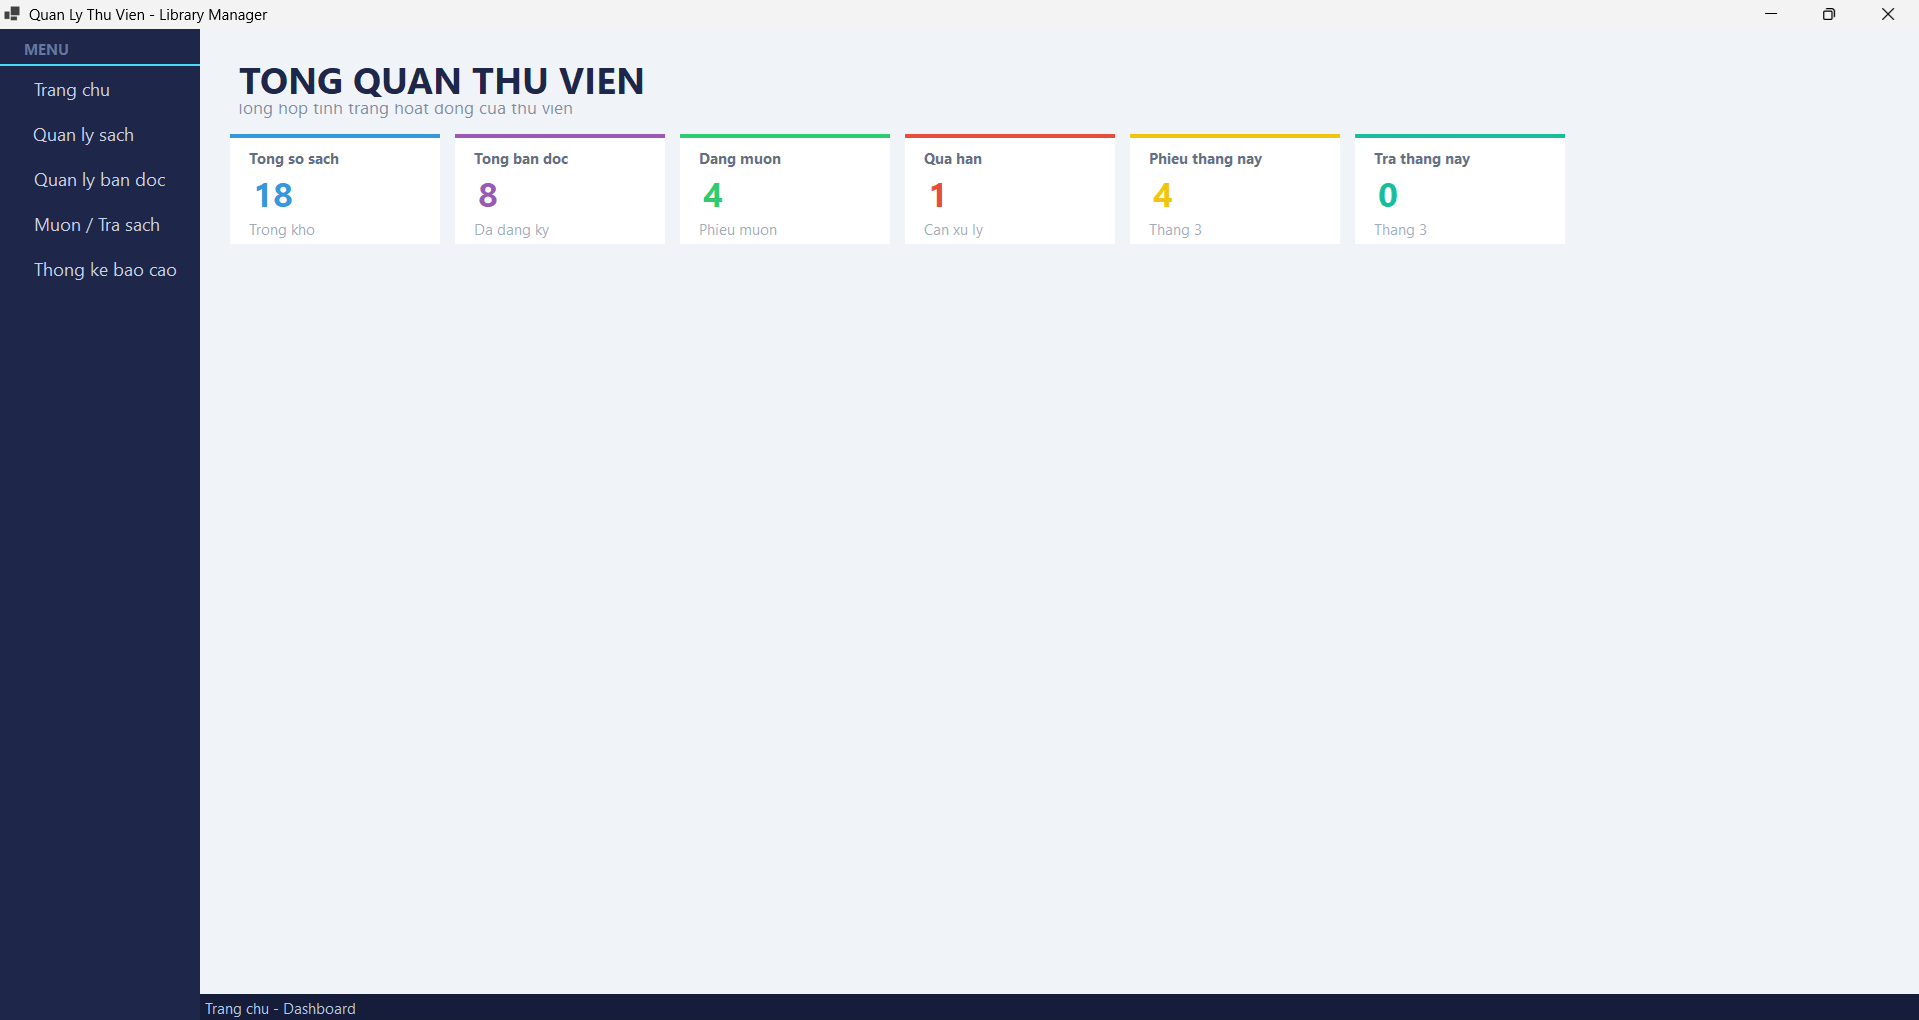
\includegraphics[width=\textwidth]{trangchu_tongquanthuvien.png}
    \caption{Dashboard tổng quan của hệ thống.}
    \label{fig:dashboard}
\end{figure}

\subsection{Nhóm chức năng quản lý sách}
\subsubsection{Danh sách sách}
Hình~\ref{fig:book_list} trình bày màn hình quản lý sách với lưới dữ liệu hiển thị đầy đủ thông tin. Thanh tìm kiếm cho phép lọc theo tên sách, thể loại và tác giả.
\begin{figure}[H]
    \centering
    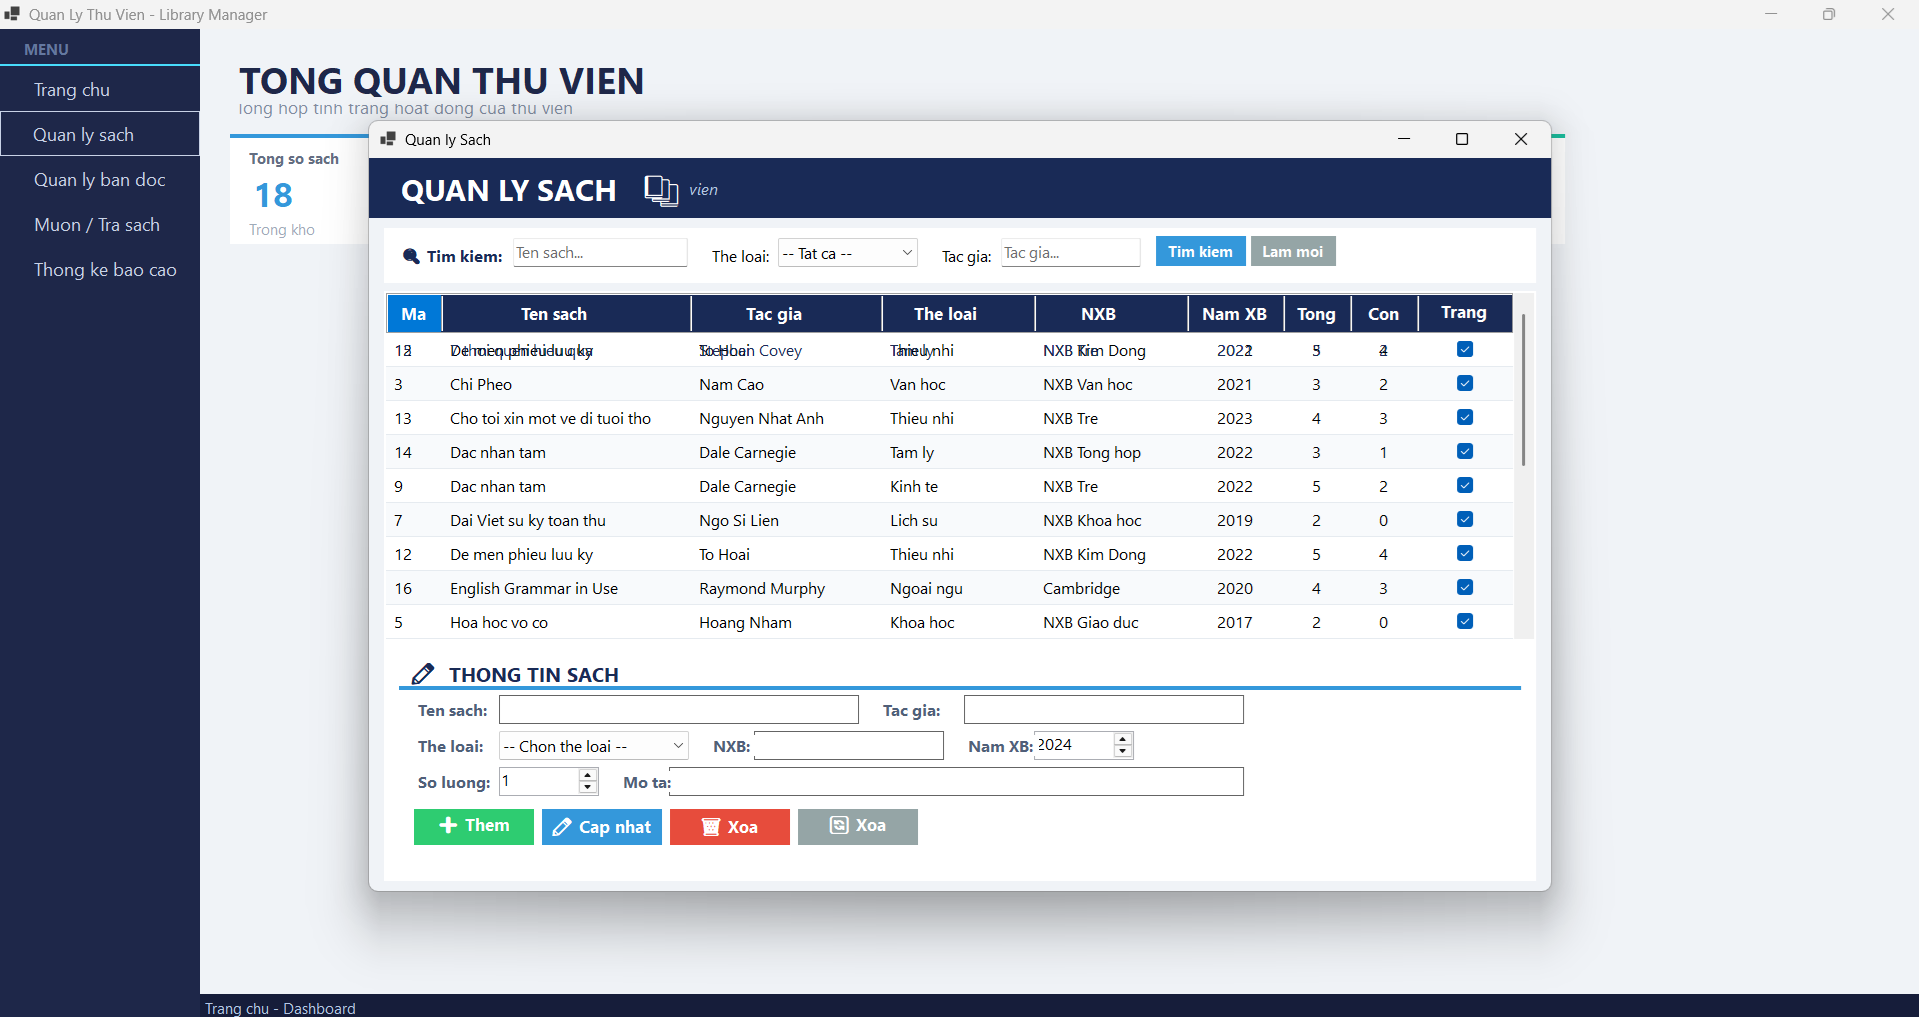
\includegraphics[width=\textwidth]{quanlysach_dashboard.png}
    \caption{Màn hình danh sách sách và form nhập liệu.}
    \label{fig:book_list}
\end{figure}

\subsubsection{Thêm sách mới}
Hình~\ref{fig:book_add} thể hiện thao tác thêm sách thành công. Hệ thống xác nhận bằng hộp thoại hiển thị mã sách được sinh tự động.
\begin{figure}[H]
    \centering
    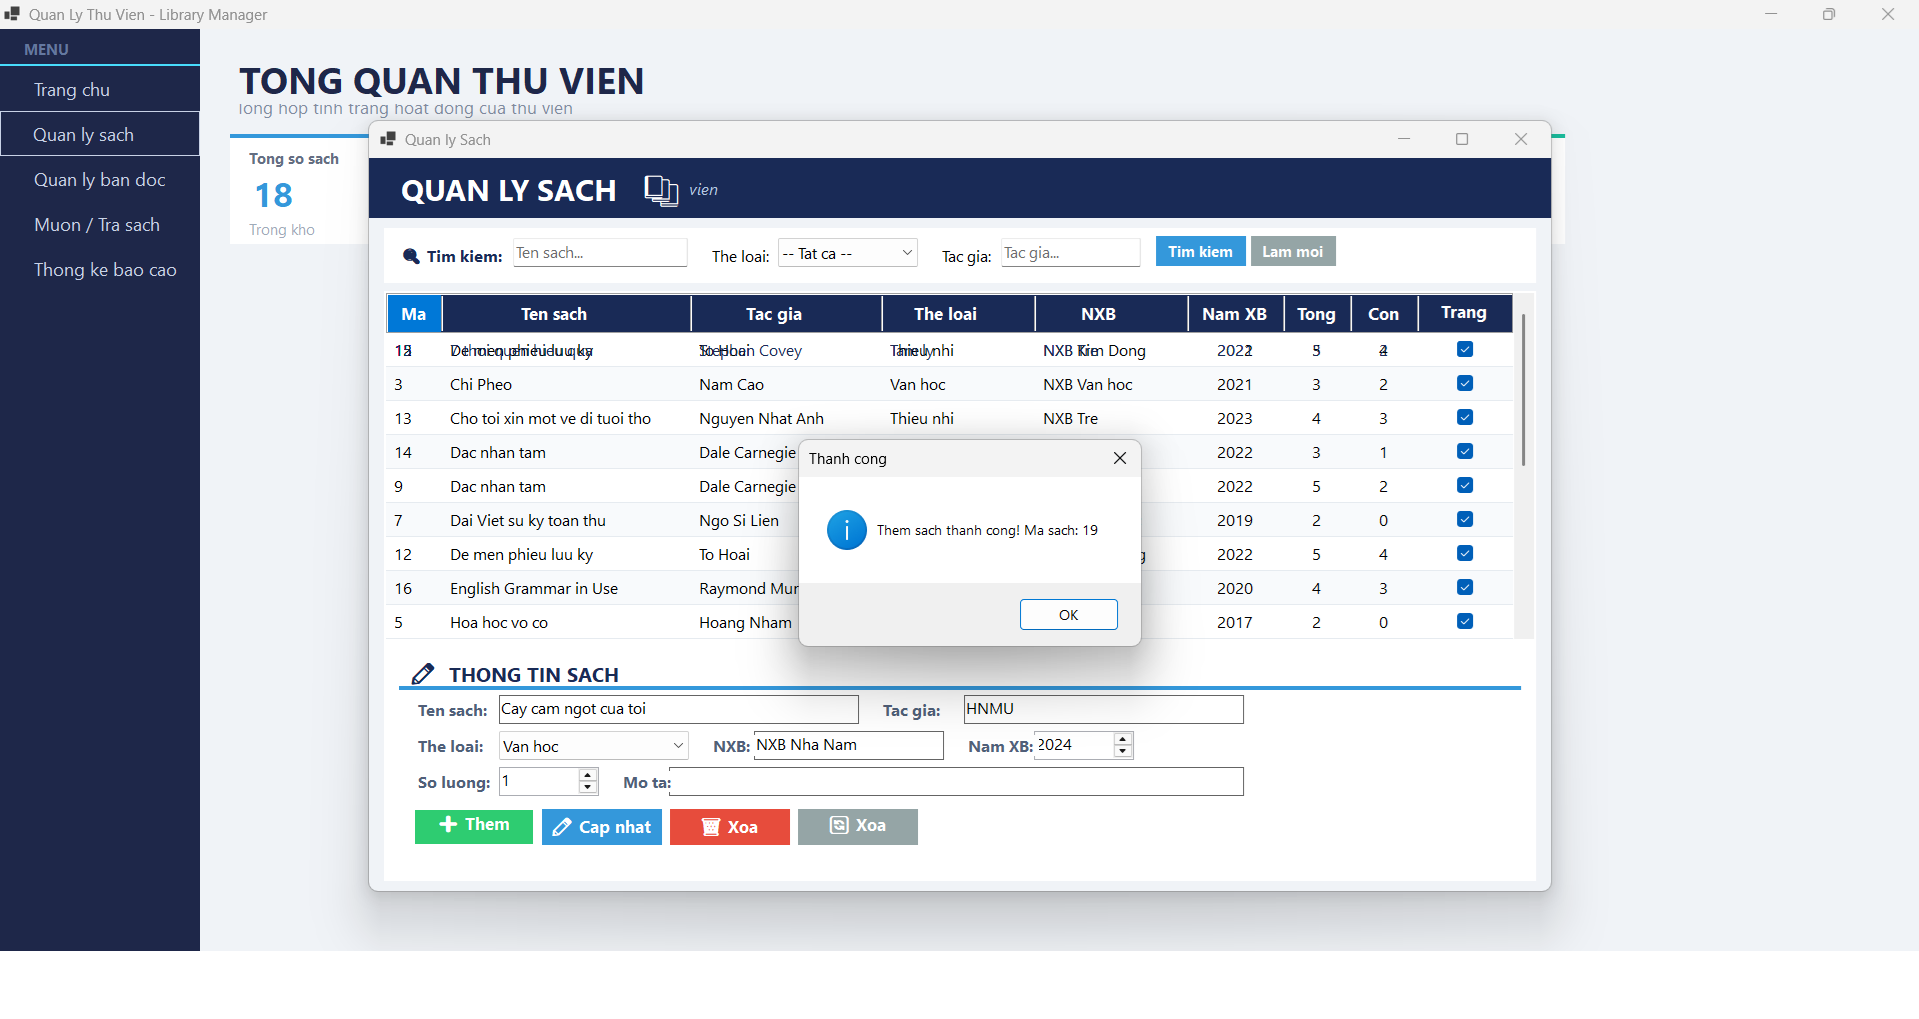
\includegraphics[width=\textwidth]{quanlysach_themsach.png}
    \caption{Thêm sách mới thành công.}
    \label{fig:book_add}
\end{figure}

\subsubsection{Cập nhật sách}
Hình~\ref{fig:book_update} minh họa thao tác cập nhật thông tin sách. Khi thay đổi số lượng tổng, số lượng còn được tính lại tự động.
\begin{figure}[H]
    \centering
    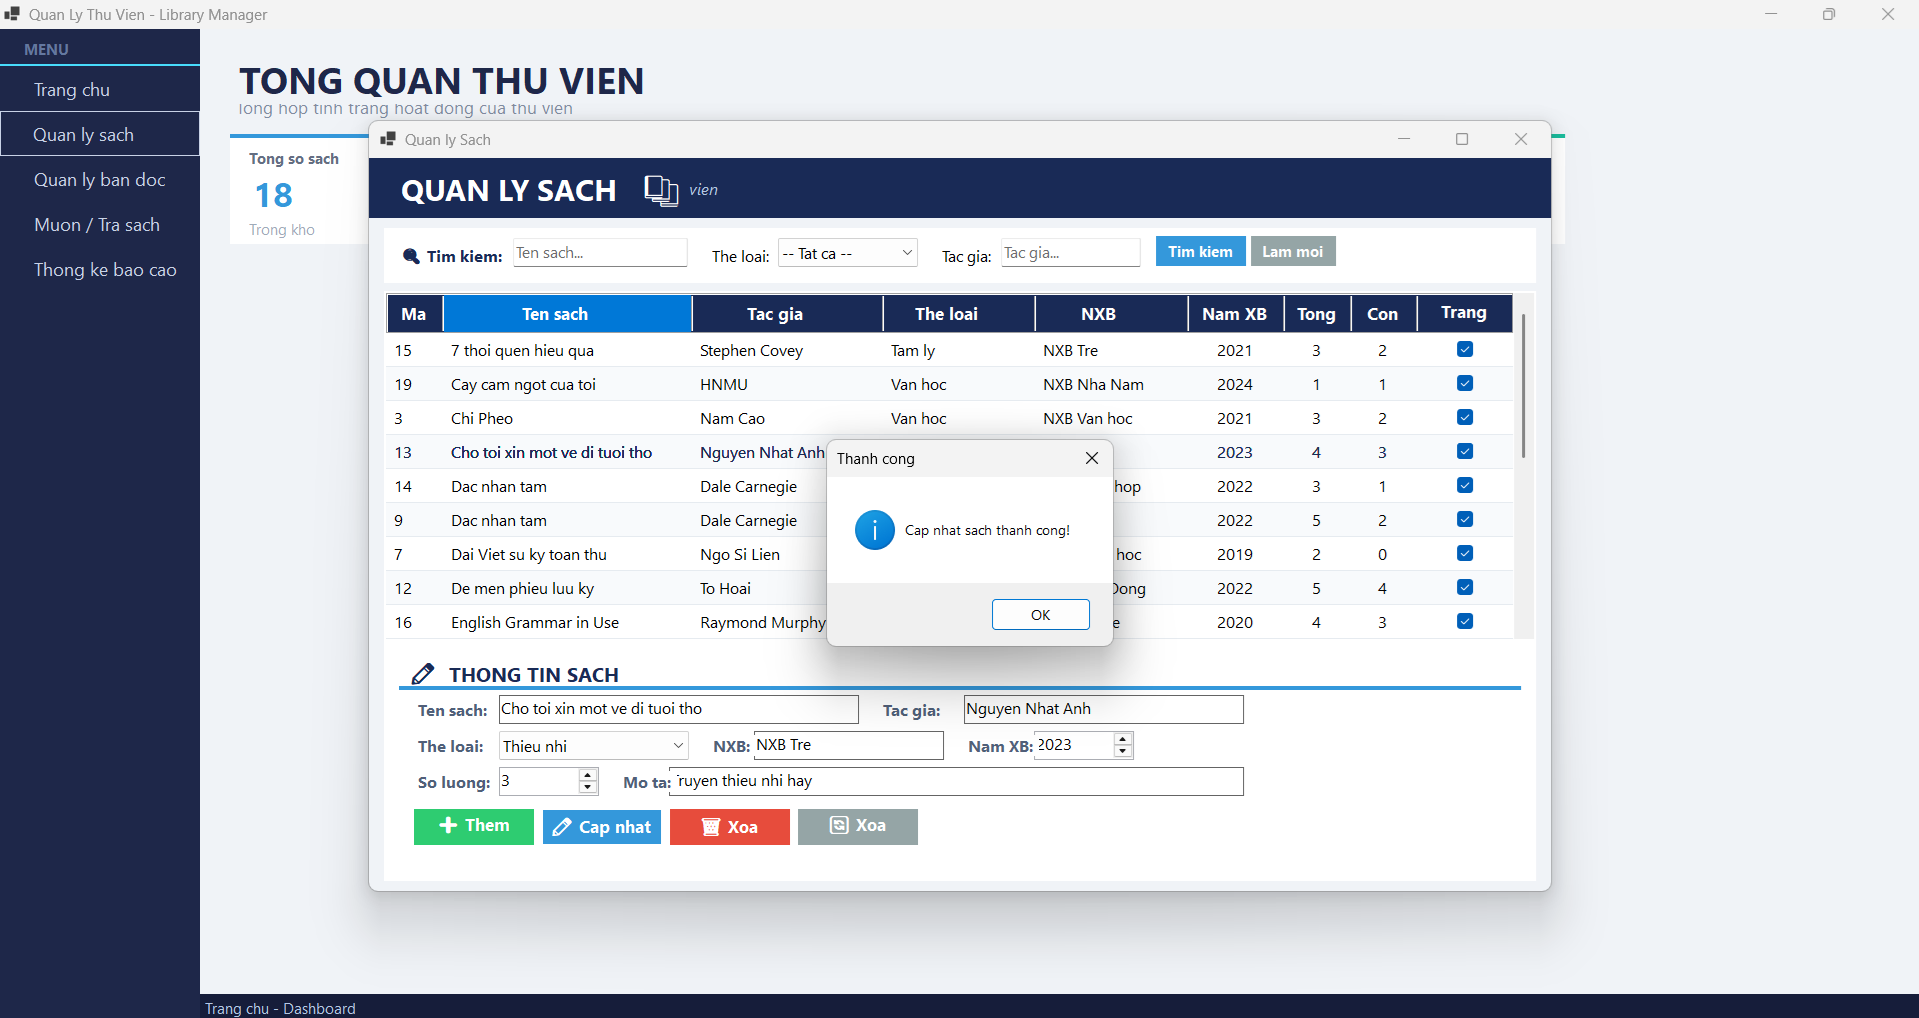
\includegraphics[width=\textwidth]{quanlysach_capnhatsach.png}
    \caption{Cập nhật thông tin sách.}
    \label{fig:book_update}
\end{figure}

\subsubsection{Xóa sách}
Hình~\ref{fig:book_delete} hiển thị hộp thoại xác nhận xóa. Nếu sách đã phát sinh mượn-trả, thao tác xóa sẽ bị chặn bởi ràng buộc khóa ngoại.
\begin{figure}[H]
    \centering
    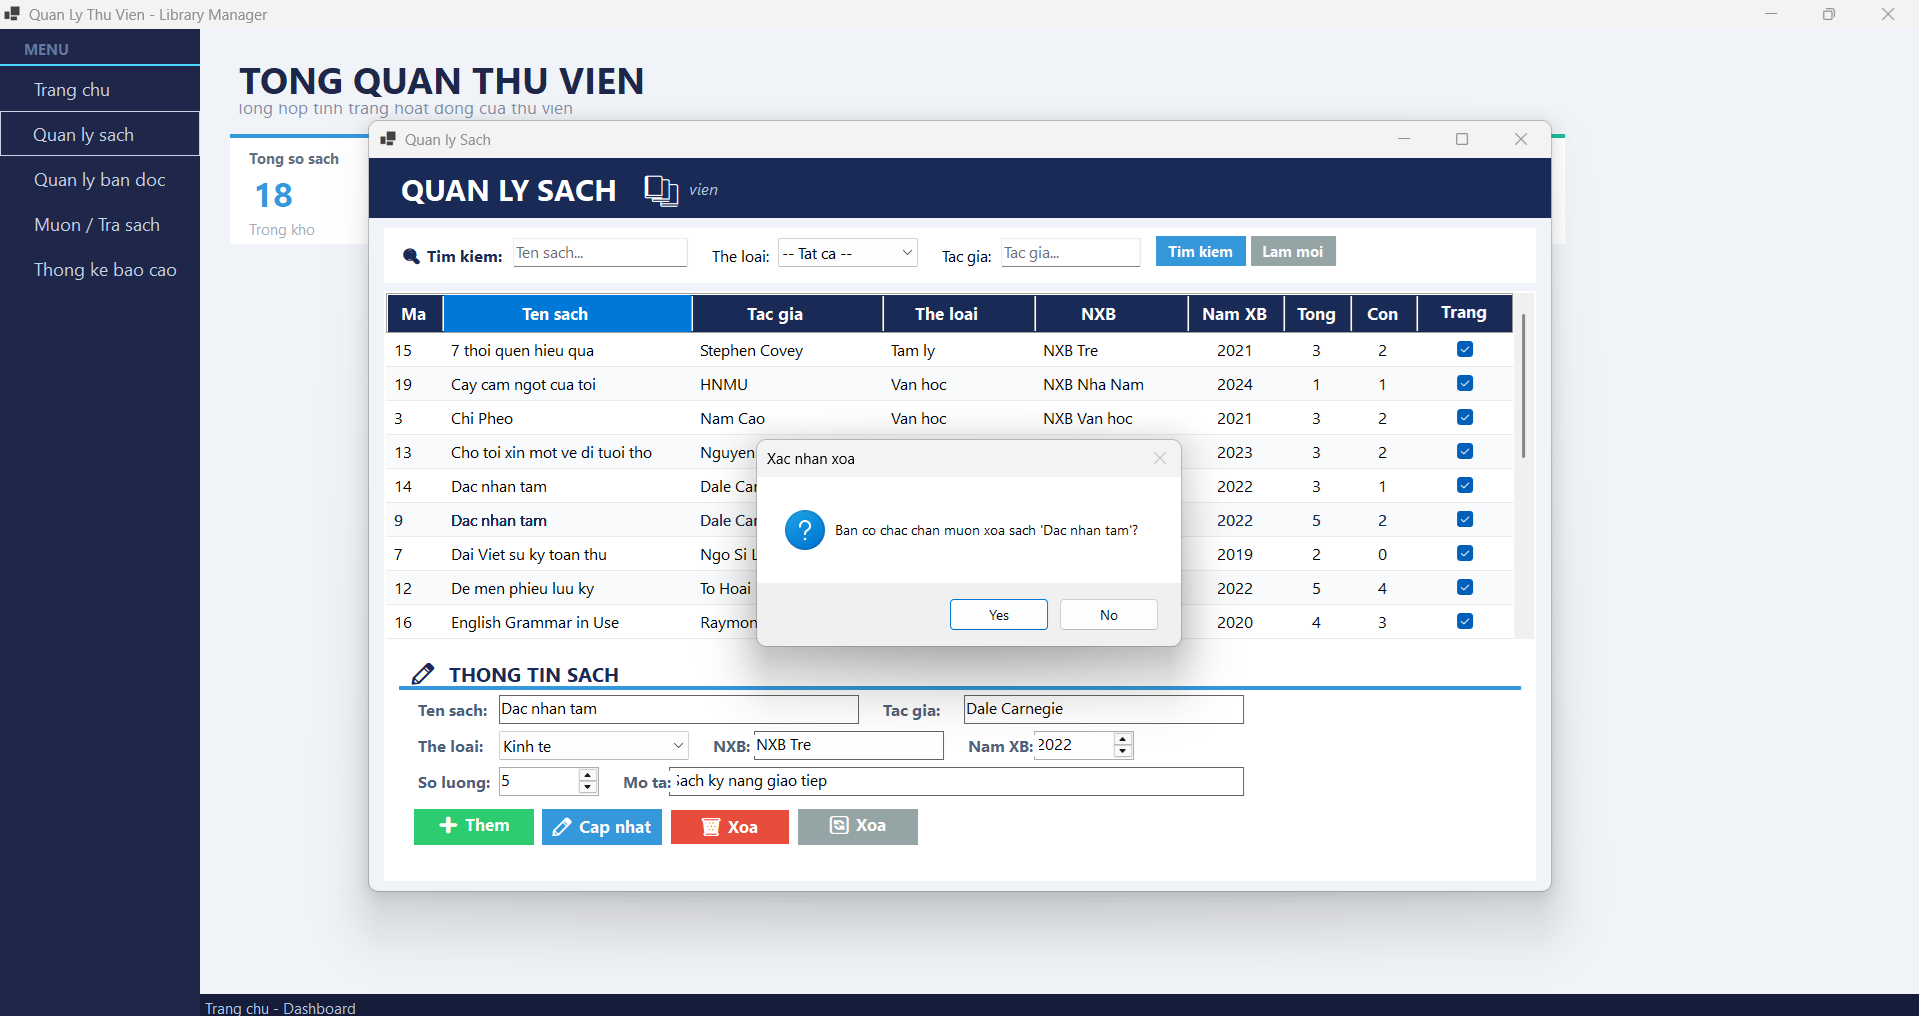
\includegraphics[width=\textwidth]{quanlysach_xoasach.png}
    \caption{Xác nhận xóa sách.}
    \label{fig:book_delete}
\end{figure}

\subsection{Nhóm chức năng quản lý bạn đọc}
\subsubsection{Danh sách bạn đọc}
\begin{figure}[H]
    \centering
    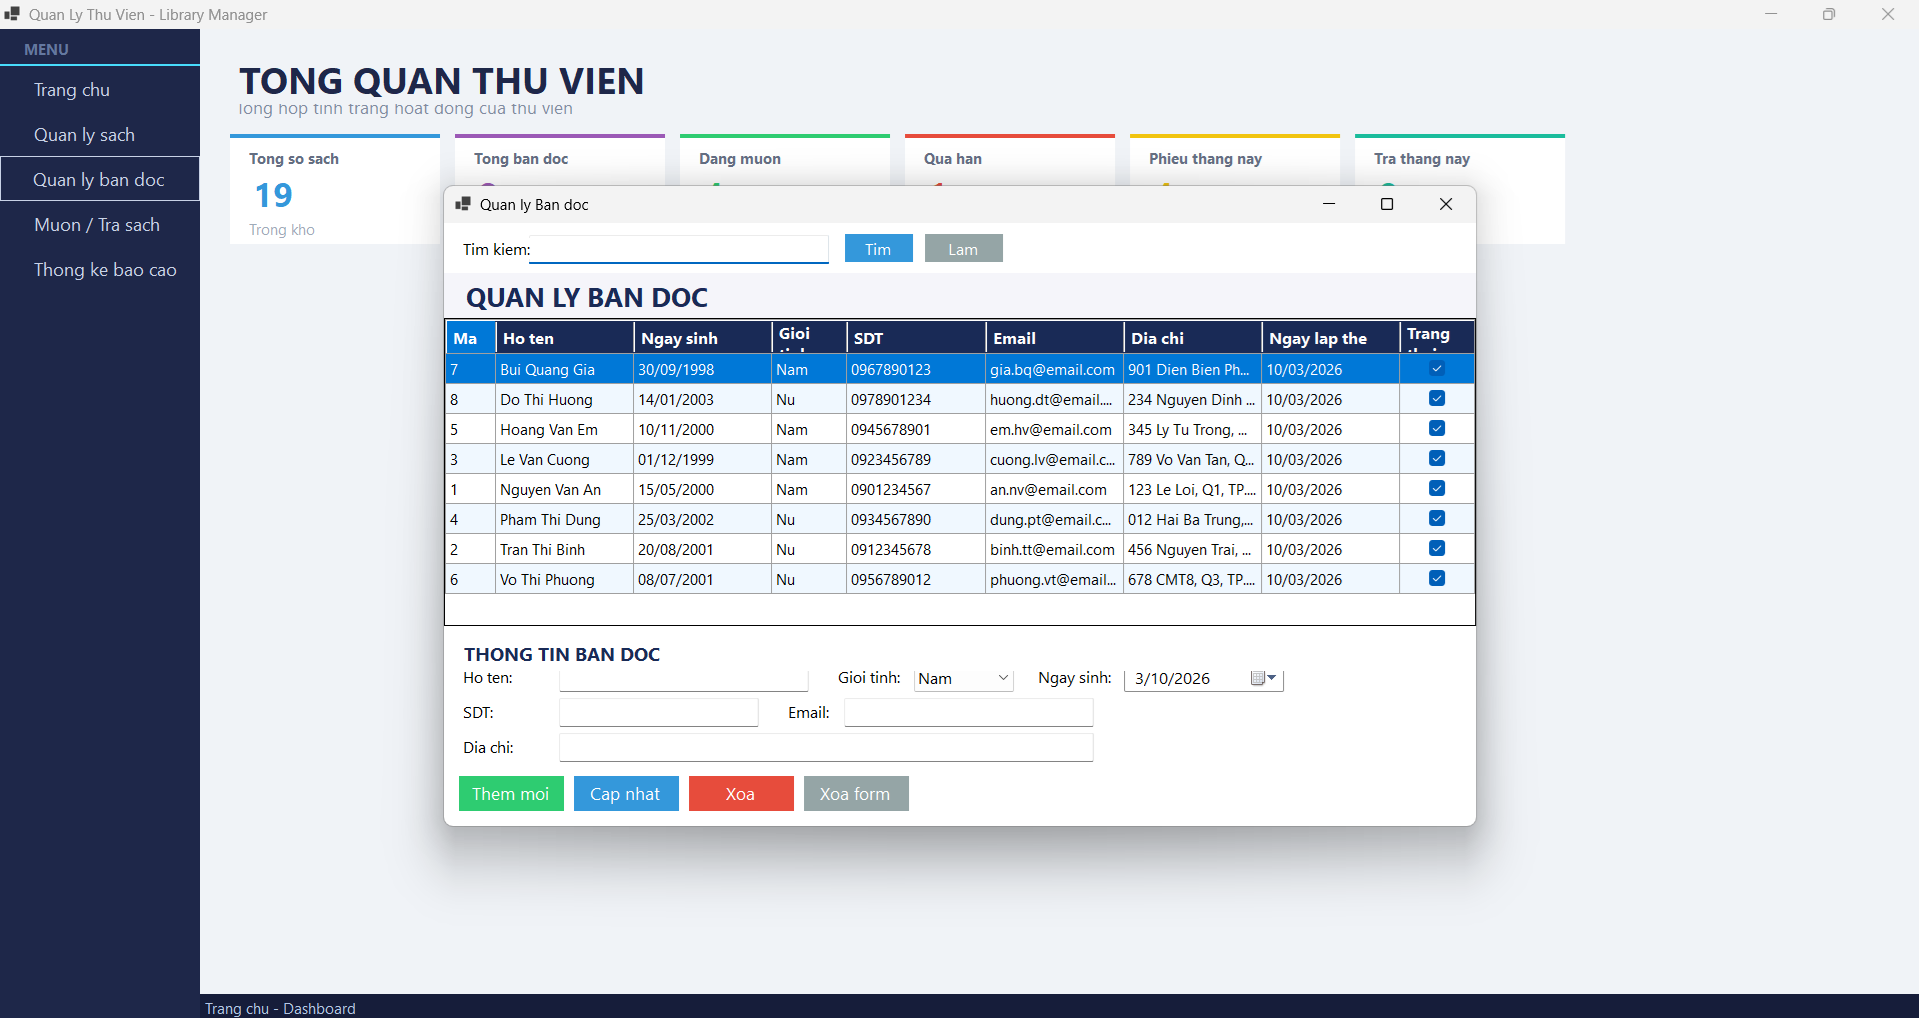
\includegraphics[width=\textwidth]{quanlybandoc_dashboard.png}
    \caption{Màn hình danh sách bạn đọc.}
    \label{fig:reader_list}
\end{figure}

\subsubsection{Thêm bạn đọc}
\begin{figure}[H]
    \centering
    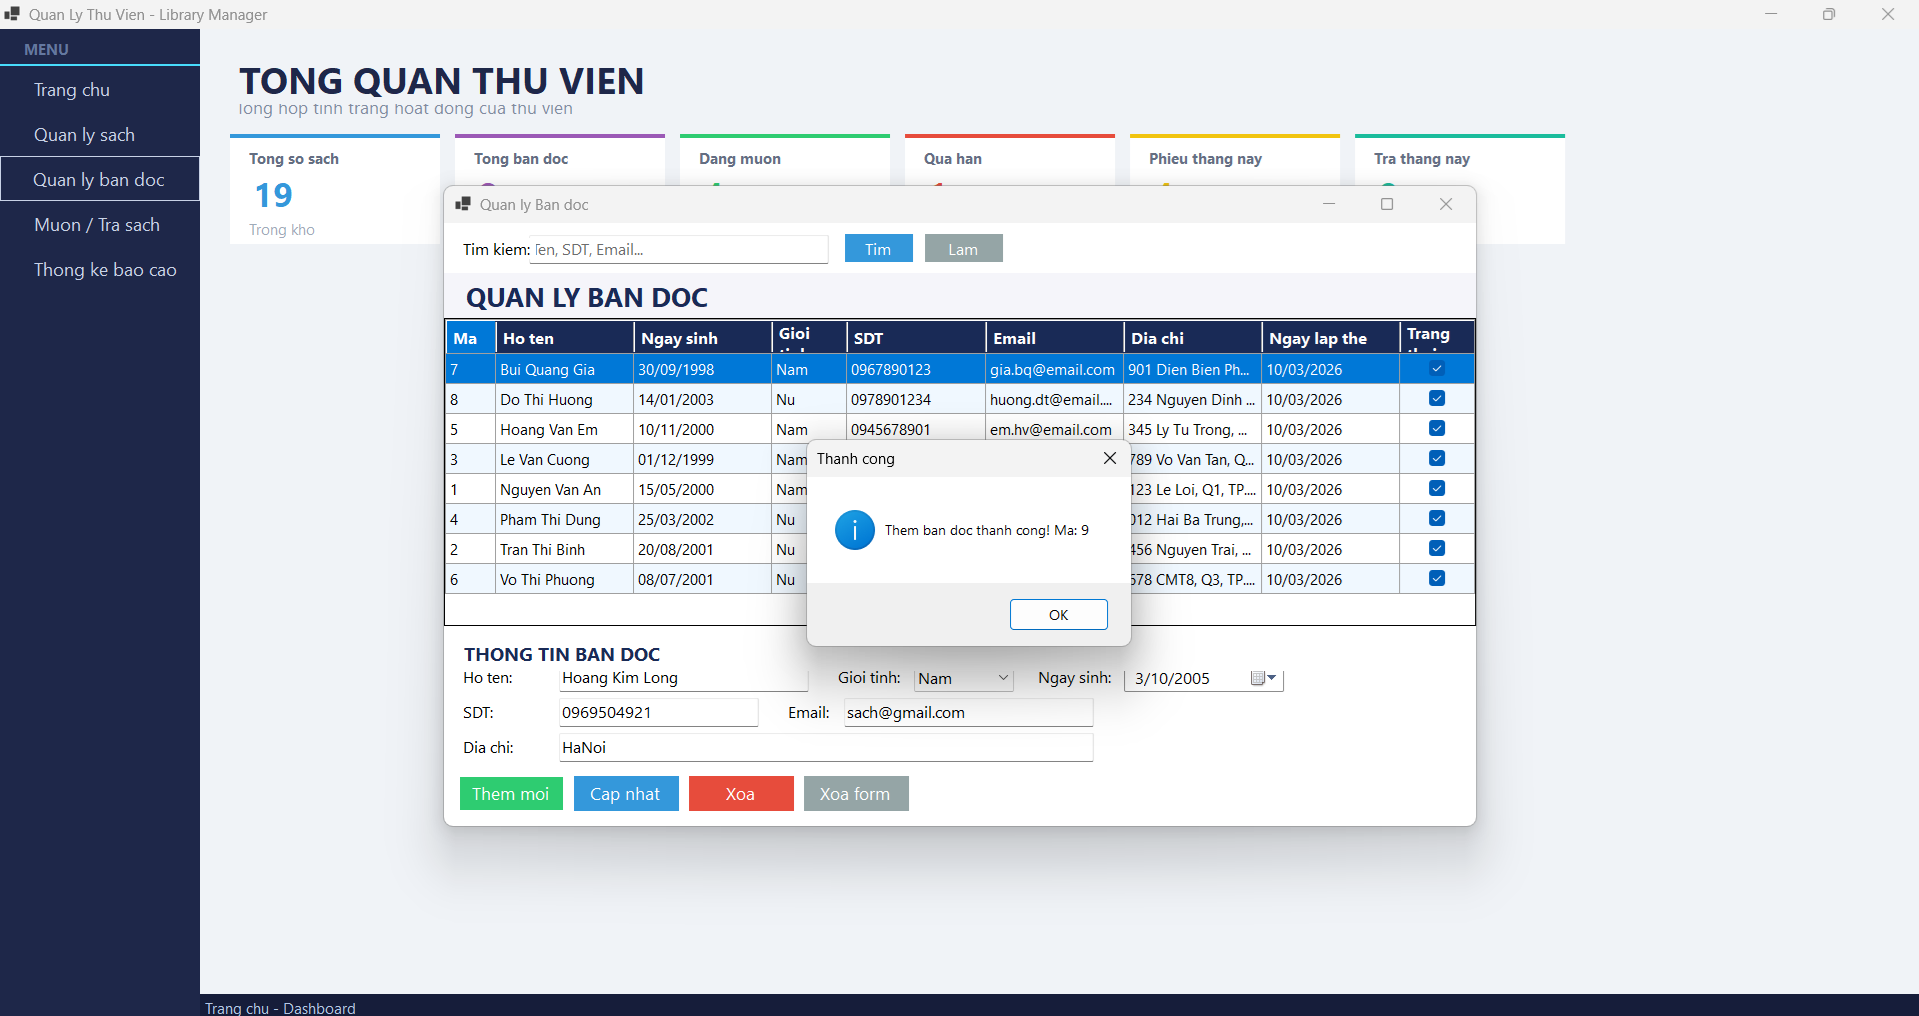
\includegraphics[width=\textwidth]{quanlybandoc_them.png}
    \caption{Thêm bạn đọc mới thành công.}
    \label{fig:reader_add}
\end{figure}

\subsubsection{Cập nhật bạn đọc}
\begin{figure}[H]
    \centering
    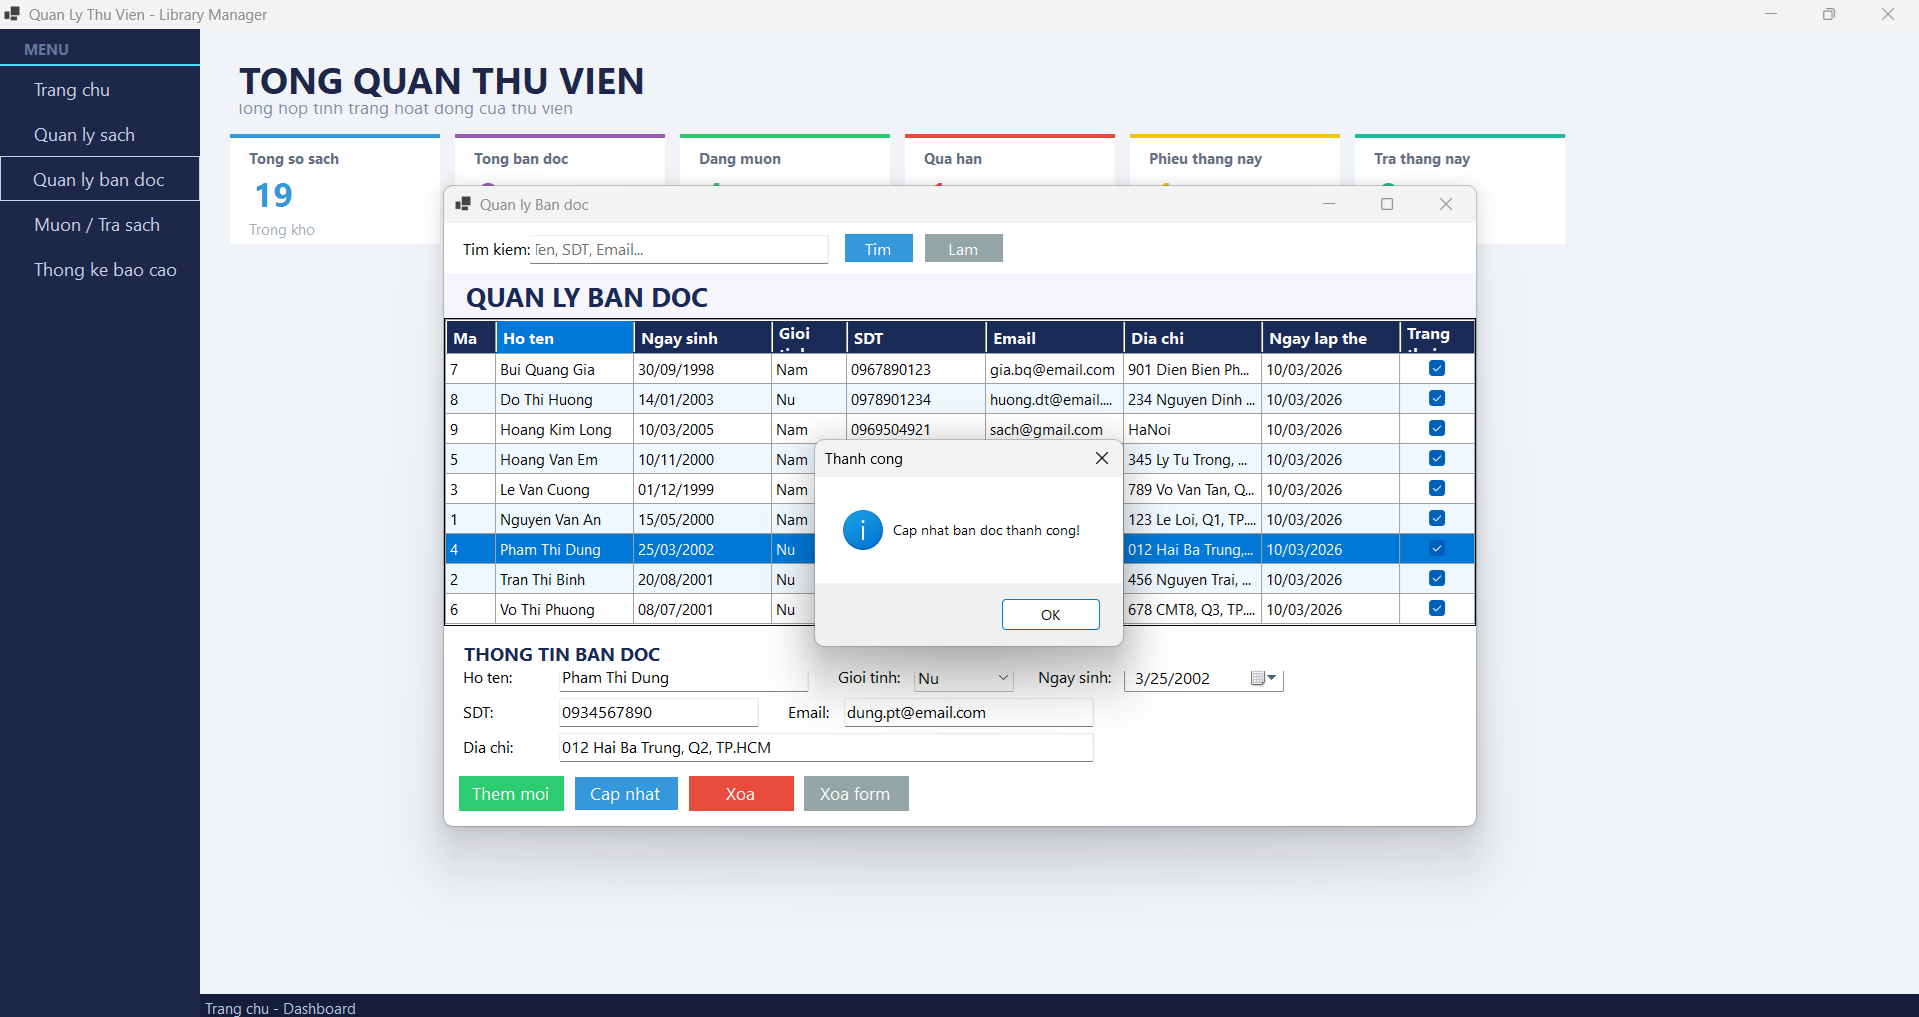
\includegraphics[width=\textwidth]{quanlybandoc_capnhat.png}
    \caption{Cập nhật thông tin bạn đọc.}
    \label{fig:reader_update}
\end{figure}

\subsubsection{Xóa bạn đọc}
Hình~\ref{fig:reader_delete}: nếu bạn đọc vẫn còn sách chưa trả, hệ thống sẽ từ chối xóa.
\begin{figure}[H]
    \centering
    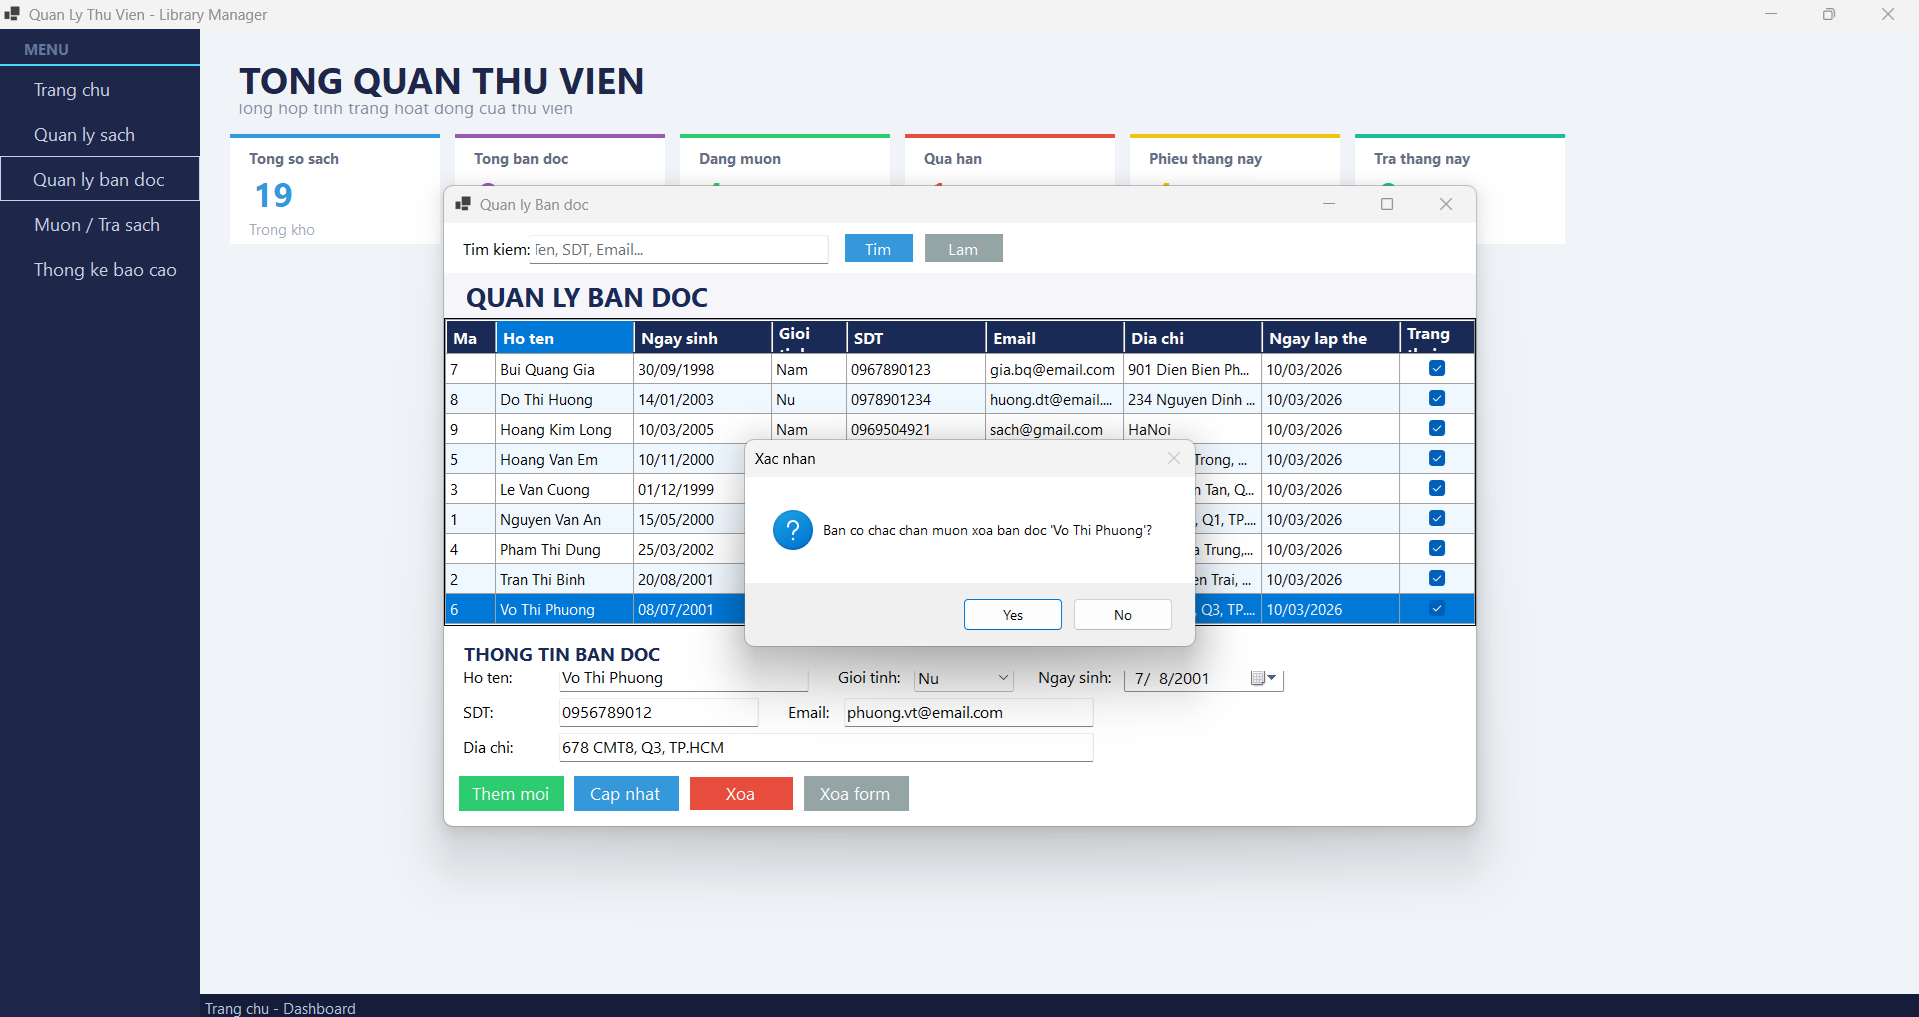
\includegraphics[width=\textwidth]{quanlybandoc_xoa.png}
    \caption{Xác nhận xóa bạn đọc.}
    \label{fig:reader_delete}
\end{figure}

\subsection{Nhóm chức năng mượn/trả}
\subsubsection{Danh sách phiếu mượn}
Hình~\ref{fig:borrow_list} hiển thị danh sách phiếu với trạng thái phân biệt bằng màu sắc: xanh (đang mượn), đỏ (quá hạn), xanh lá (đã trả).
\begin{figure}[H]
    \centering
    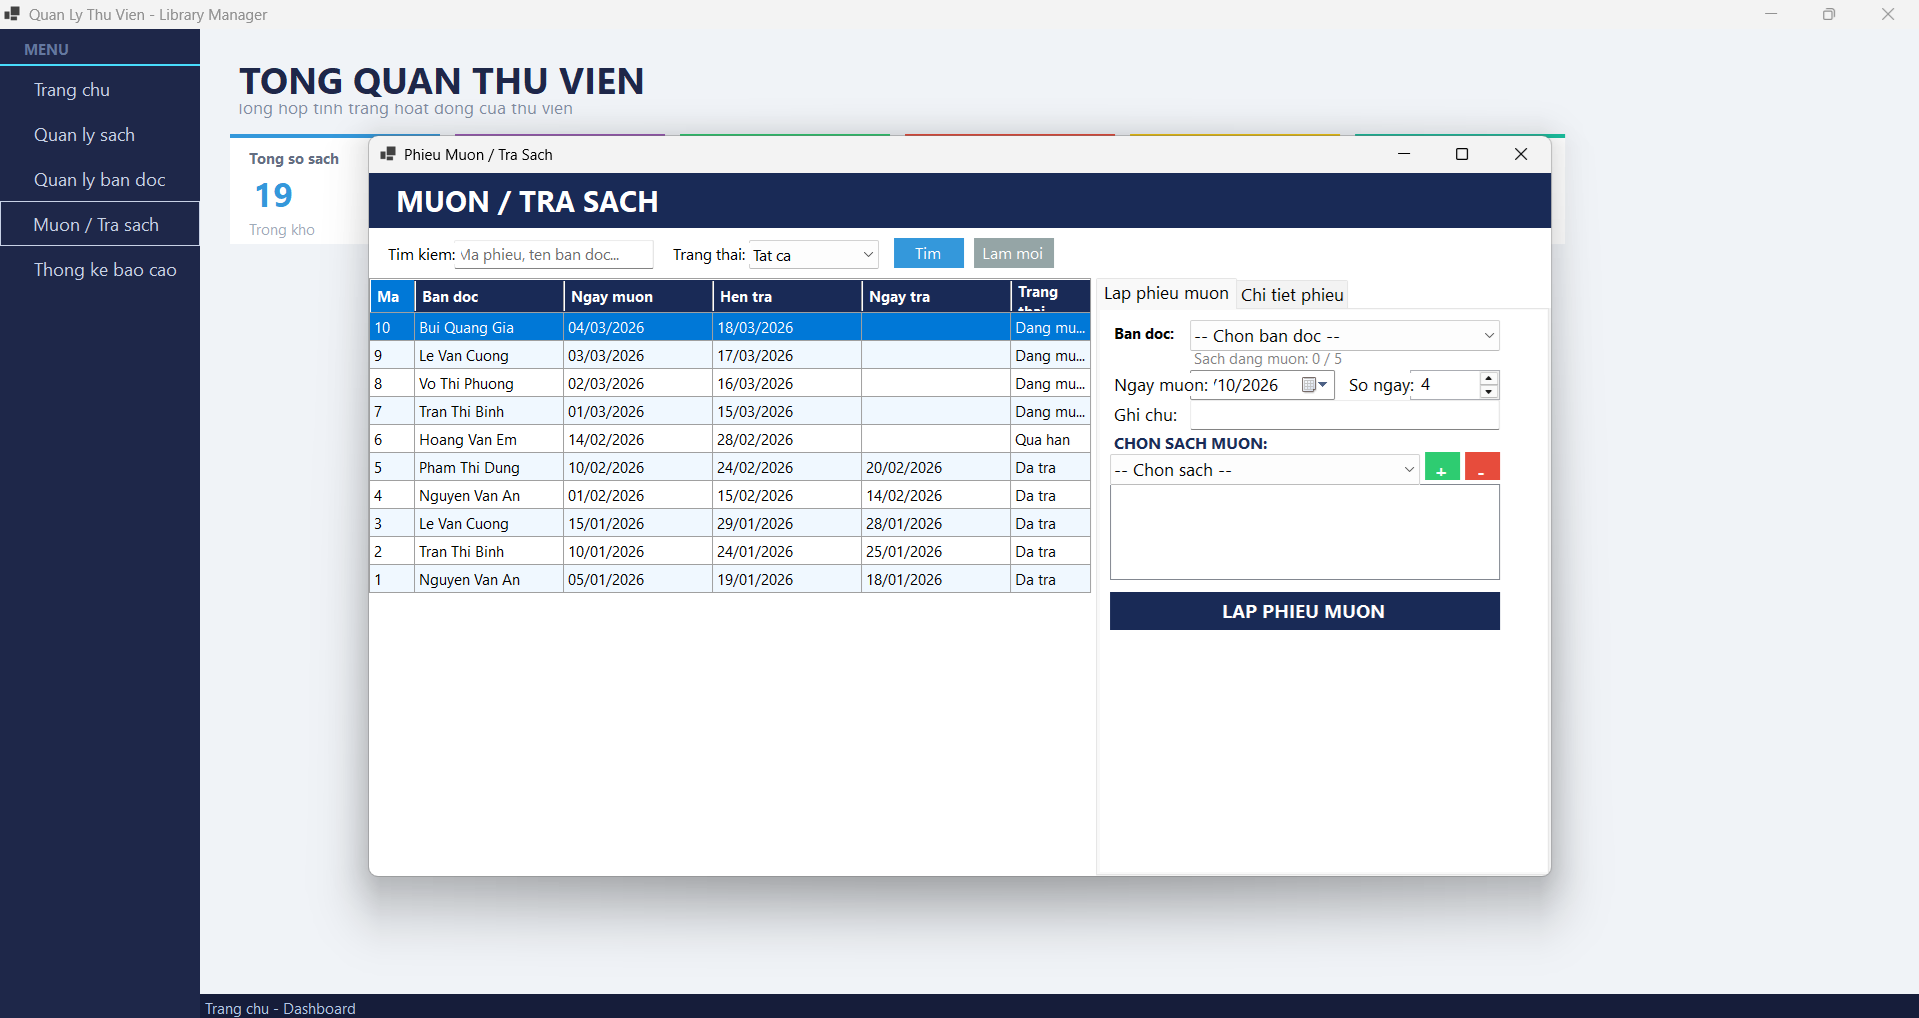
\includegraphics[width=\textwidth]{muontrasach_dashboard.png}
    \caption{Danh sách phiếu mượn và trạng thái.}
    \label{fig:borrow_list}
\end{figure}

\subsubsection{Lập phiếu mượn}
Hình~\ref{fig:borrow_create} thể hiện thao tác lập phiếu mượn thành công. Hệ thống kiểm tra số sách đang mượn trước khi cho phép tạo phiếu.
\begin{figure}[H]
    \centering
    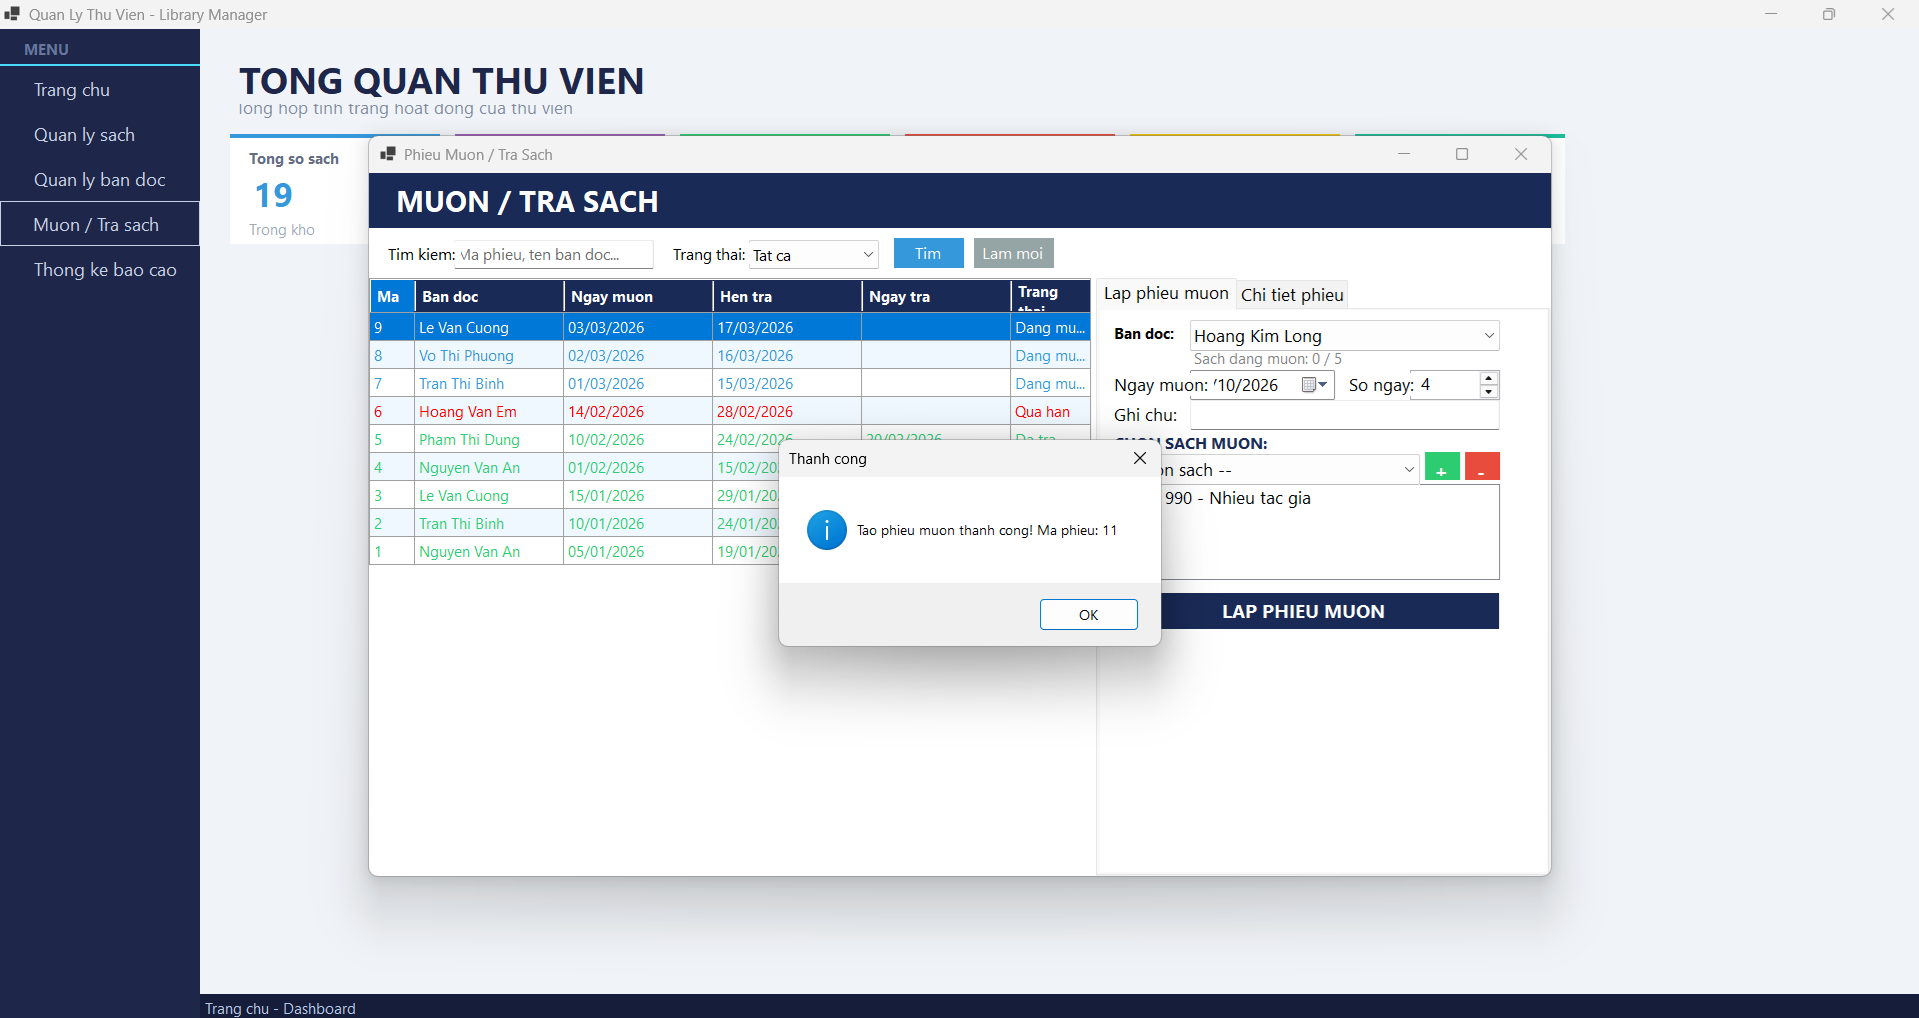
\includegraphics[width=\textwidth]{muontrasach_lapphieumuon.png}
    \caption{Lập phiếu mượn thành công.}
    \label{fig:borrow_create}
\end{figure}

\subsubsection{Xác nhận trả sách}
Hình~\ref{fig:return_confirm} minh họa hộp thoại xác nhận trước khi thực thi thao tác trả sách.
\begin{figure}[H]
    \centering
    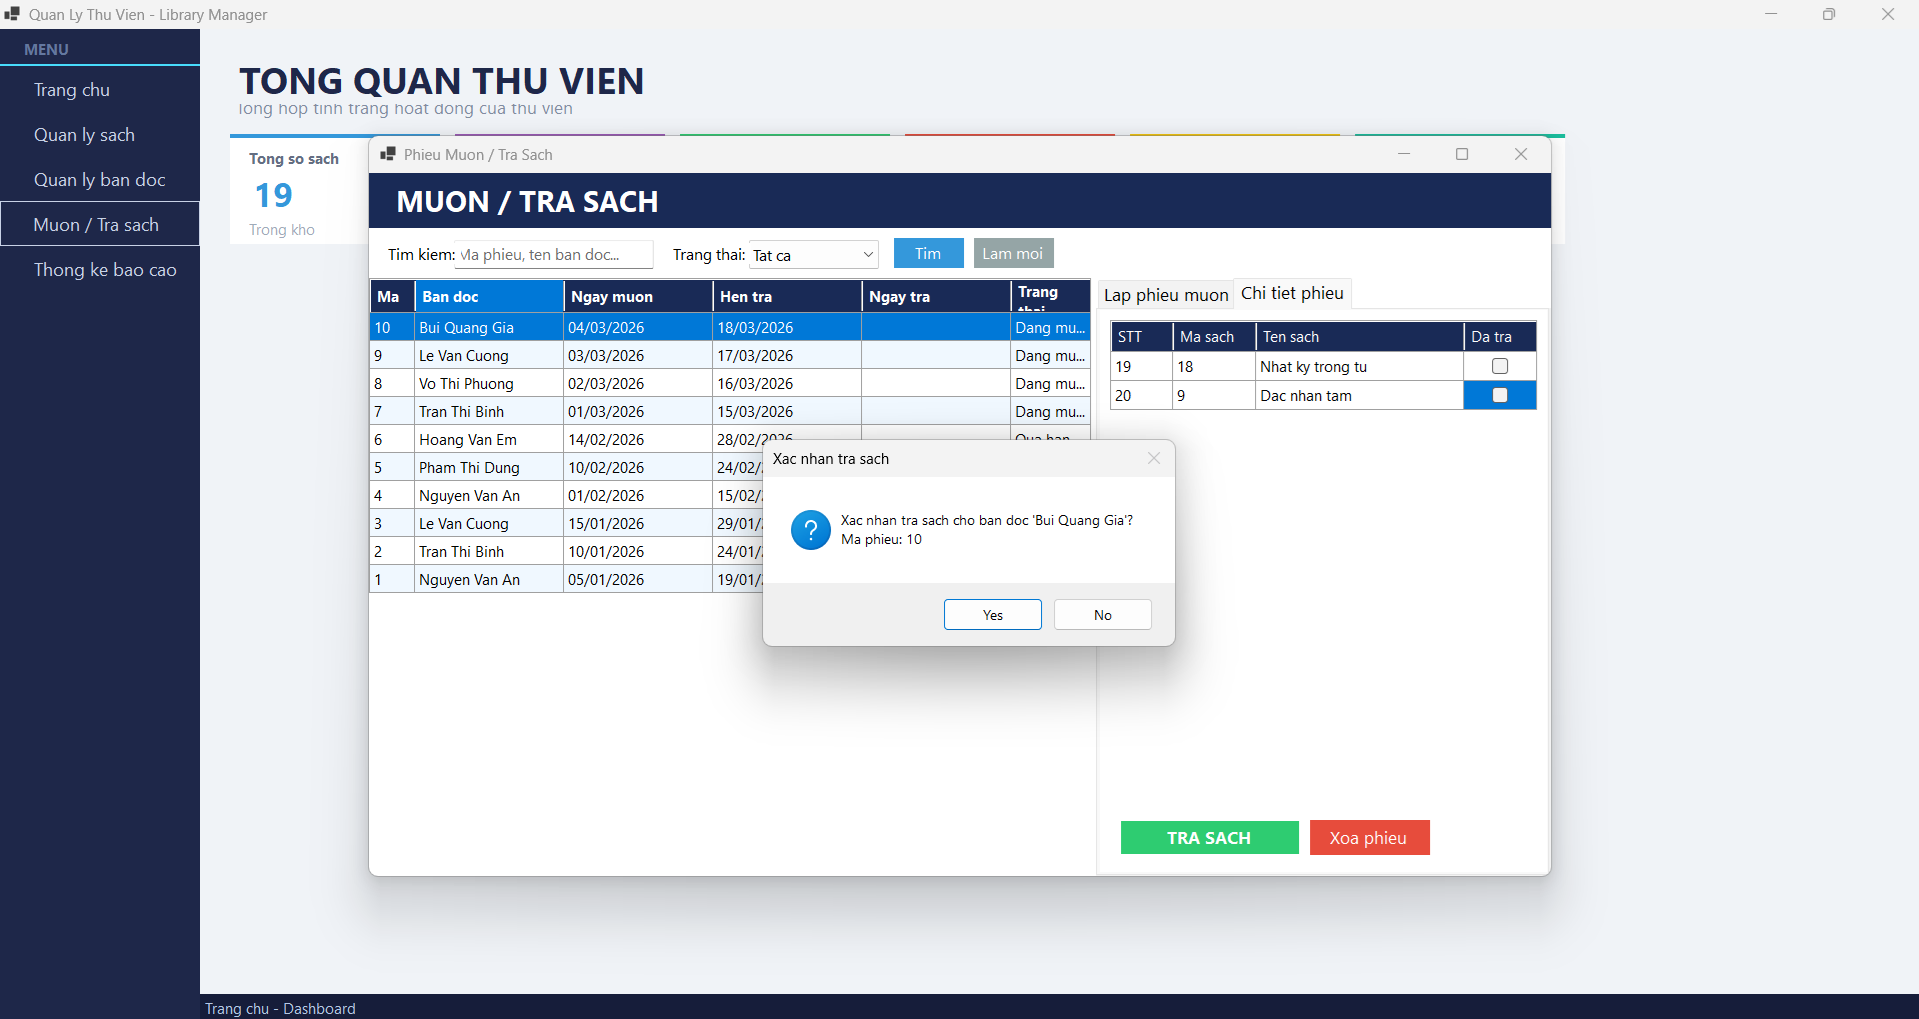
\includegraphics[width=\textwidth]{muontrasach_trasach.png}
    \caption{Xác nhận trả sách.}
    \label{fig:return_confirm}
\end{figure}

\subsubsection{Trả sách thành công}
Hình~\ref{fig:return_success}: sau khi trả, trạng thái phiếu chuyển thành ``Đã trả'', tồn kho được cộng lại đúng.
\begin{figure}[H]
    \centering
    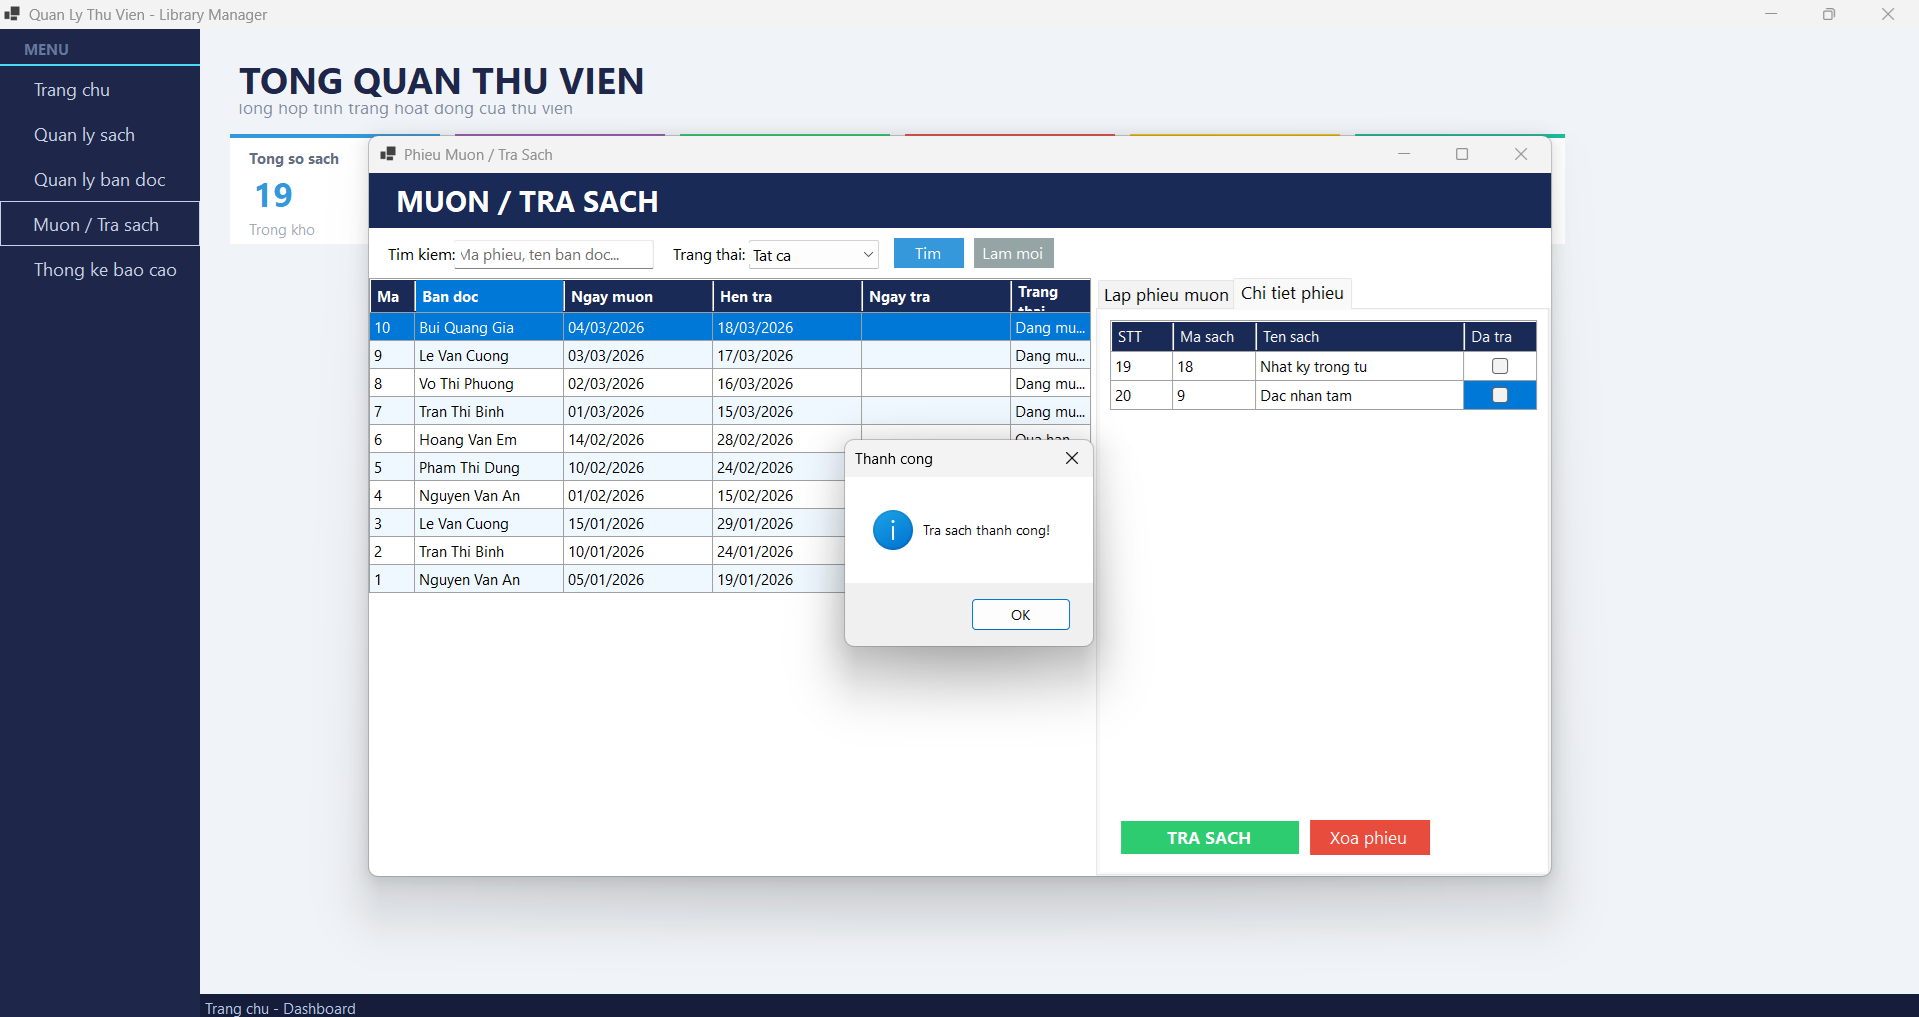
\includegraphics[width=\textwidth]{muontrasach_trasach_thanhcong.png}
    \caption{Trả sách thành công.}
    \label{fig:return_success}
\end{figure}

\subsubsection{Xóa phiếu đã hoàn tất}
\begin{figure}[H]
    \centering
    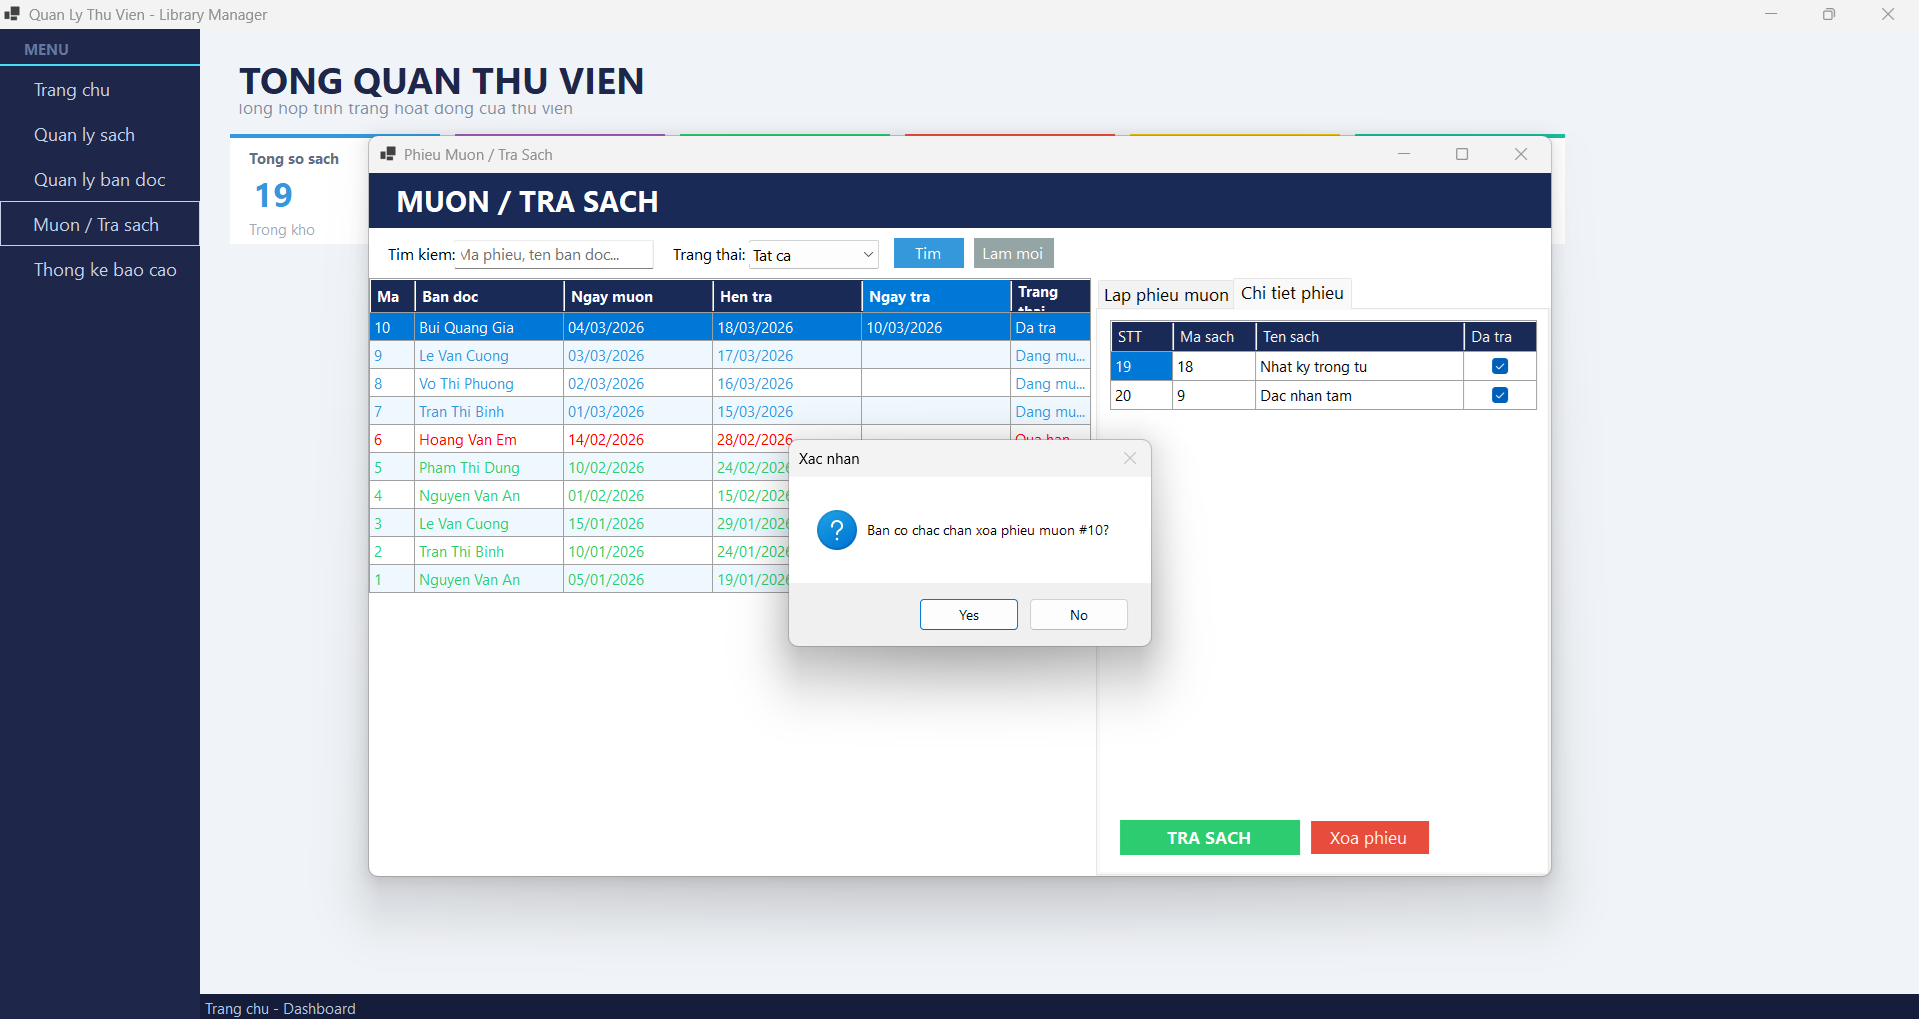
\includegraphics[width=\textwidth]{muontrasach_xoaphieu.png}
    \caption{Xóa phiếu đã hoàn tất trả sách.}
    \label{fig:ticket_delete}
\end{figure}

\subsection{Nhóm chức năng thống kê và báo cáo}
\subsubsection{Màn hình thống kê}
Hình~\ref{fig:stats_dashboard} hiển thị thống kê mượn/trả theo tháng, bảng xu hướng theo các tháng trong năm và danh sách sách mượn nhiều nhất.
\begin{figure}[H]
    \centering
    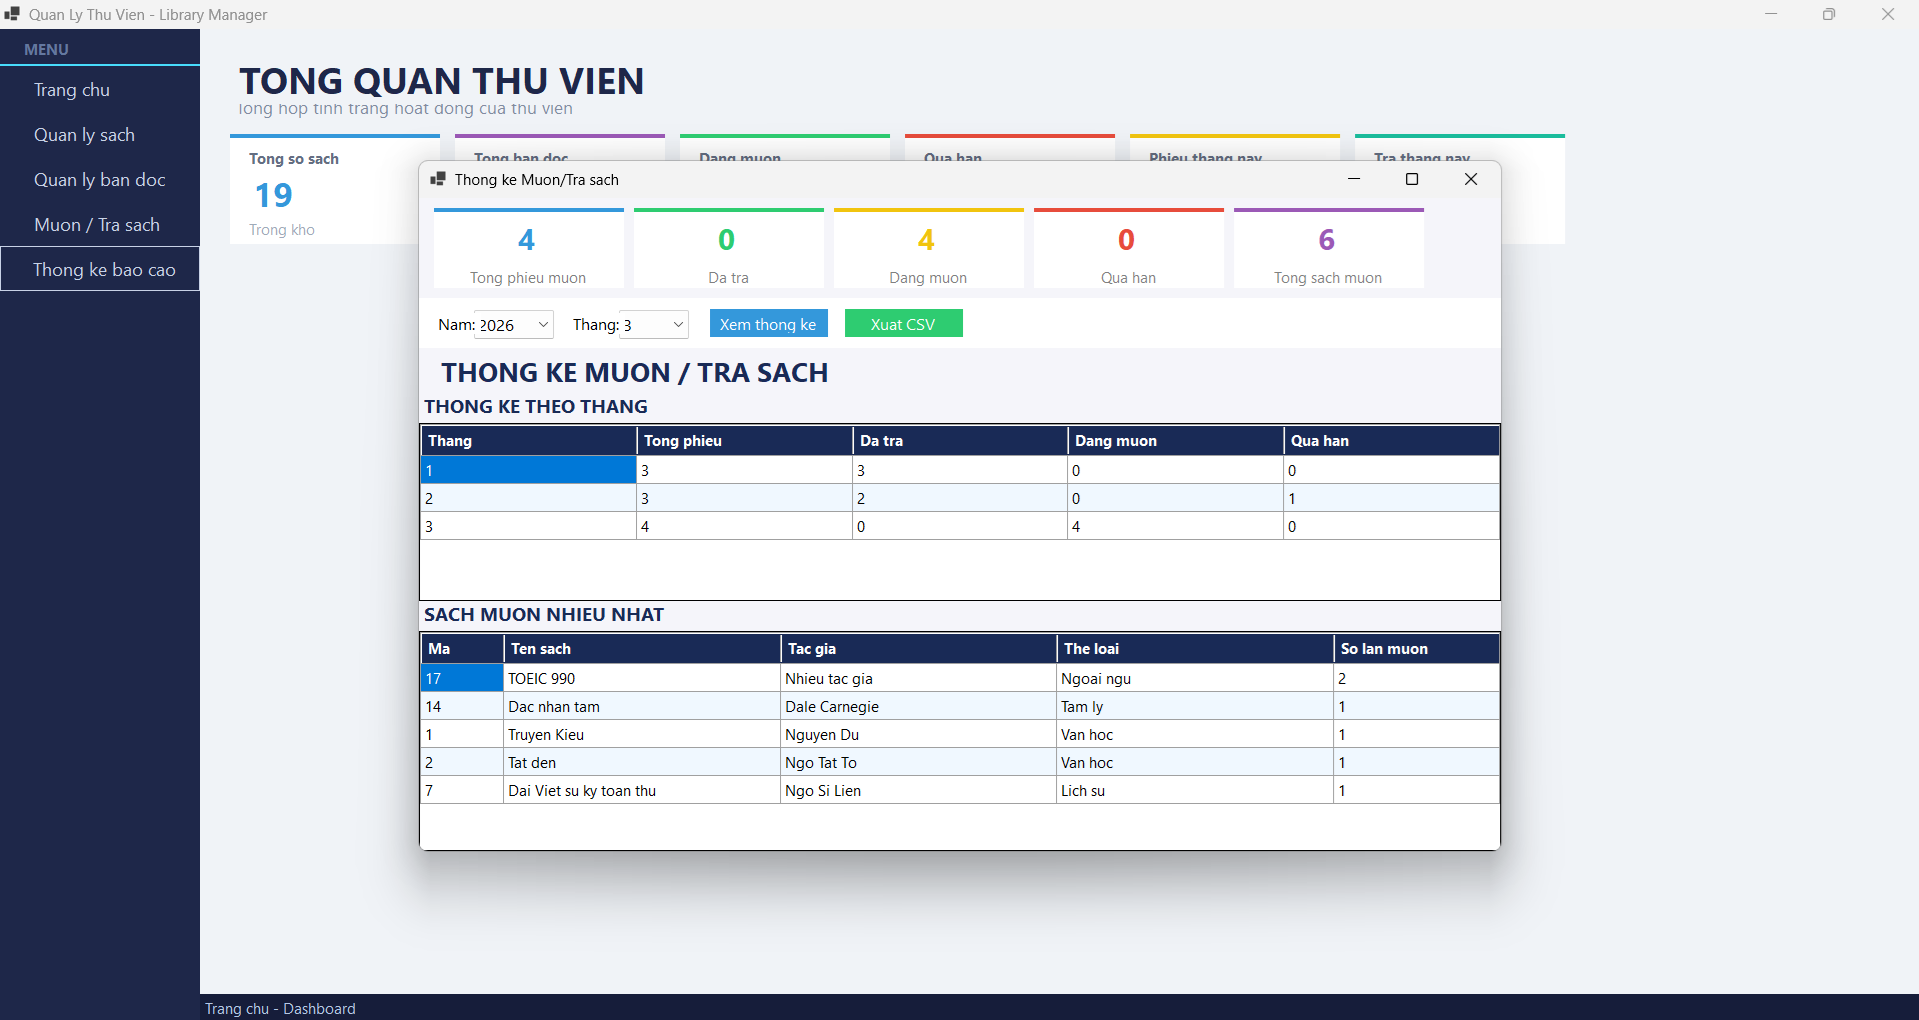
\includegraphics[width=\textwidth]{thongkebaocao_dashboard.png}
    \caption{Thống kê mượn/trả theo tháng và top sách mượn nhiều.}
    \label{fig:stats_dashboard}
\end{figure}

\subsubsection{Xuất báo cáo CSV}
\begin{figure}[H]
    \centering
    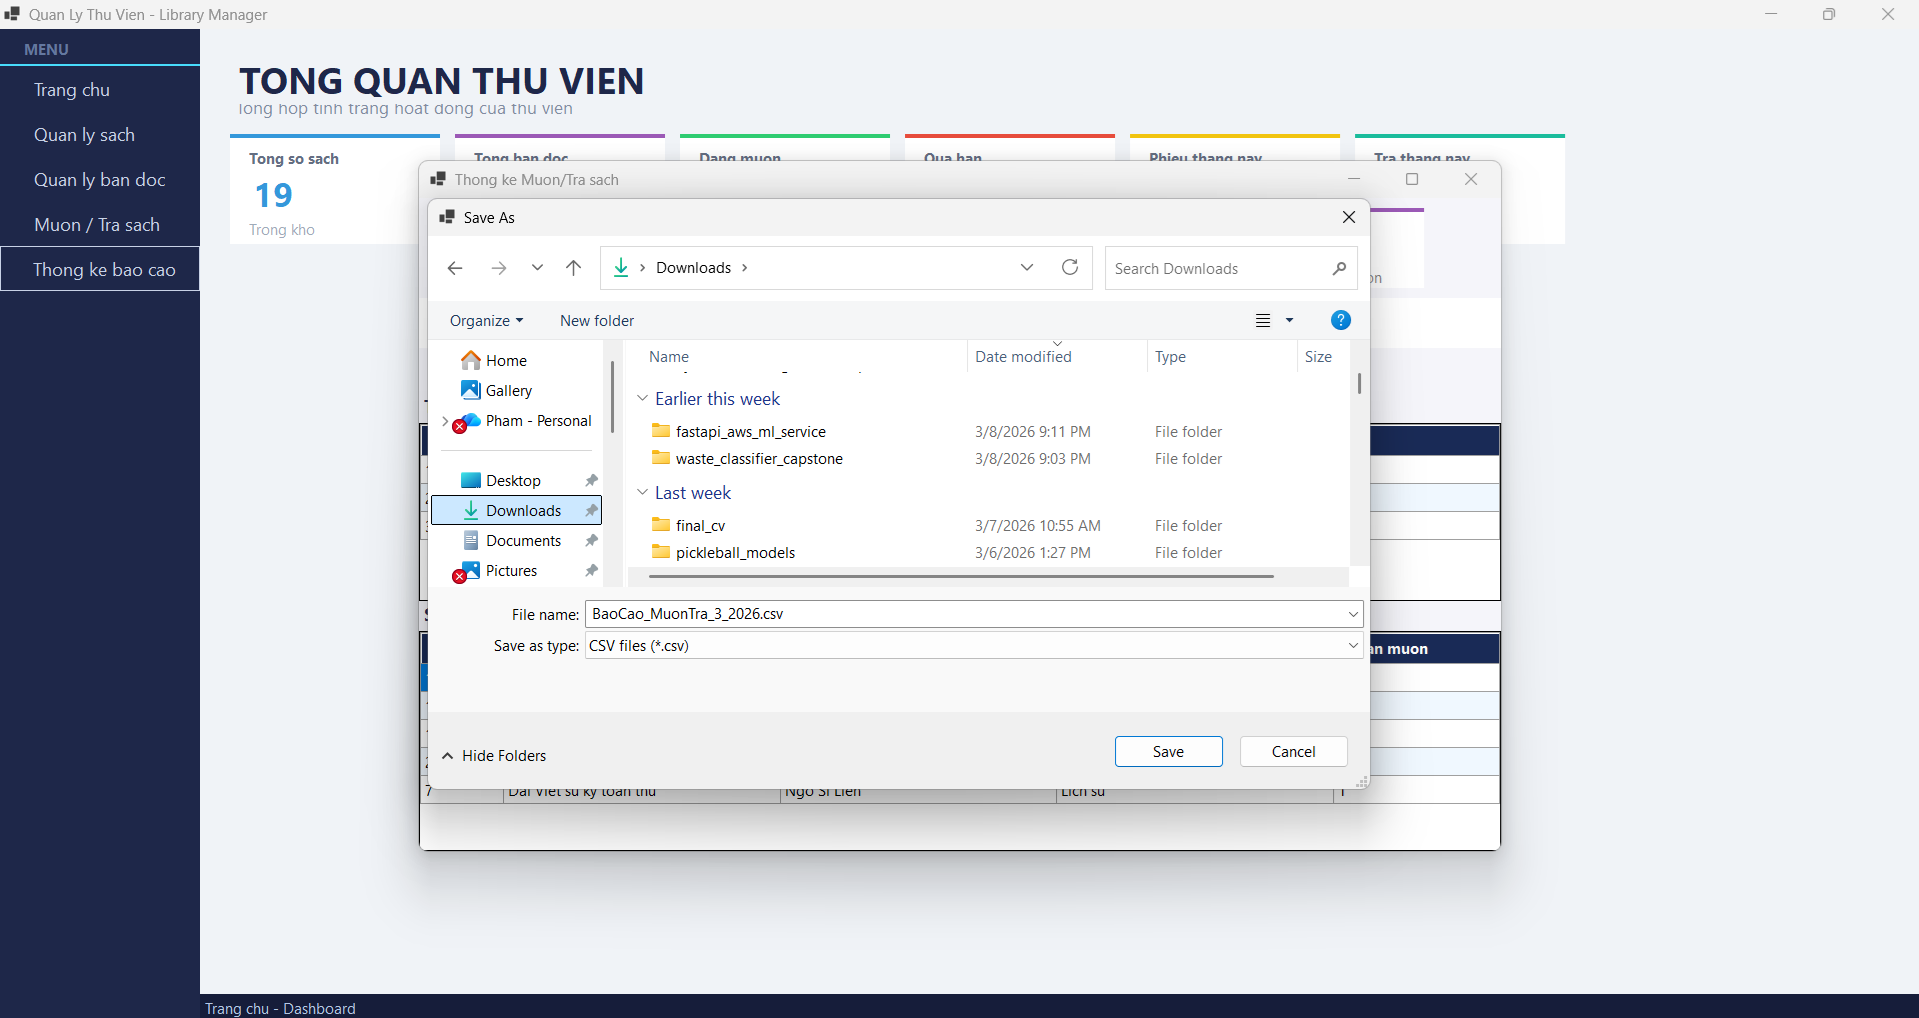
\includegraphics[width=\textwidth]{thongkebaocao_xuatcsv.png}
    \caption{Hộp thoại xuất báo cáo CSV.}
    \label{fig:csv_export}
\end{figure}

\subsection{Đối chiếu yêu cầu chức năng}
\begin{table}[H]
\centering
\caption{Đối chiếu yêu cầu chức năng và hình minh chứng.}
\label{tab:fr_coverage}
\begin{tabularx}{\textwidth}{p{1.5cm}p{5.5cm}X}
\toprule
\textbf{FR} & \textbf{Yêu cầu} & \textbf{Hình minh chứng} \\
\midrule
FR1 & Quản lý sách và thể loại & Hình~\ref{fig:book_list}, \ref{fig:book_add}, \ref{fig:book_update}, \ref{fig:book_delete} \\
FR2 & Quản lý bạn đọc & Hình~\ref{fig:reader_list}, \ref{fig:reader_add}, \ref{fig:reader_update}, \ref{fig:reader_delete} \\
FR3 & Lập phiếu mượn & Hình~\ref{fig:borrow_list}, \ref{fig:borrow_create} \\
FR4 & Xử lý trả sách & Hình~\ref{fig:return_confirm}, \ref{fig:return_success} \\
FR5 & Nhận diện quá hạn & Hình~\ref{fig:borrow_list} \\
FR6 & Thống kê báo cáo & Hình~\ref{fig:dashboard}, \ref{fig:stats_dashboard} \\
FR7 & Xuất báo cáo CSV & Hình~\ref{fig:csv_export} \\
\bottomrule
\end{tabularx}
\end{table}

% ===================== ĐÁNH GIÁ =====================
\section{Đánh giá thực nghiệm}
\subsection{Môi trường kiểm thử}
\begin{itemize}[leftmargin=1.5cm]
    \item Hệ điều hành: Windows 10/11;
    \item IDE: Visual Studio 2022;
    \item .NET 6 SDK;
    \item SQL Server Express.
\end{itemize}

\subsection{Bộ dữ liệu mẫu}
Script khởi tạo CSDL cung cấp bộ dữ liệu mẫu gồm 8 thể loại, 18 đầu sách, 8 bạn đọc, 10 phiếu mượn và 20 dòng chi tiết mượn. Phân bổ trạng thái: 5 phiếu đã trả, 4 phiếu đang mượn, 1 phiếu quá hạn.

\subsection{Các ca kiểm thử đại diện}
\begin{longtable}{p{1.2cm}p{6.0cm}p{5.4cm}p{2.0cm}}
\toprule
\textbf{ID} & \textbf{Kịch bản} & \textbf{Kết quả mong đợi} & \textbf{KQ} \\
\midrule
\endhead
TC01 & Tạo phiếu mượn hợp lệ & Tạo thành công, tồn kho giảm đúng & Đạt \\
TC02 & Mượn vượt 5 sách đang mượn & Hệ thống chặn và báo lỗi & Đạt \\
TC03 & Mượn sách hết tồn & Từ chối thao tác & Đạt \\
TC04 & Trả phiếu có nhiều sách & Cập nhật nhất quán toàn bộ & Đạt \\
TC05 & Xóa bạn đọc còn sách chưa trả & Không cho phép xóa & Đạt \\
TC06 & Xuất CSV theo tháng & File mở đúng trên Excel UTF-8 & Đạt \\
\bottomrule
\end{longtable}

\subsection{Chỉ số định lượng}
Từ dữ liệu mẫu:
\begin{align}
    \text{Tỷ lệ đã trả} &= \frac{5}{10} = 50\% \\
    \text{Tỷ lệ đang mượn} &= \frac{4}{10} = 40\% \\
    \text{Tỷ lệ quá hạn} &= \frac{1}{10} = 10\%
\end{align}

% ===================== KẾT LUẬN =====================
\section{Kết luận và hướng phát triển}
\subsection{Kết luận}
Hệ thống đã đáp ứng các nghiệp vụ quản lý thư viện cốt lõi, vận hành ổn định với dữ liệu mẫu và thể hiện rõ tính nhất quán dữ liệu trong các quy trình quan trọng. Kiến trúc phân tầng giúp mã nguồn dễ đọc, dễ bảo trì và thuận lợi mở rộng.

\subsection{Hướng phát triển}
\begin{itemize}[leftmargin=1.5cm]
    \item Bổ sung đăng nhập, phân quyền theo vai trò;
    \item Bổ sung nhật ký thao tác (audit log);
    \item Tích hợp nhắc quá hạn qua email;
    \item Tích hợp barcode/QR;
    \item Mở rộng thành REST API cho web/mobile.
\end{itemize}

% ===================== LỜI CẢM ƠN =====================
\section*{Lời cảm ơn}
\addcontentsline{toc}{section}{Lời cảm ơn}
Nhóm xin chân thành cảm ơn Khoa Công nghệ thông tin đã hỗ trợ trong quá trình thực hiện và đánh giá dự án.

% ===================== TÀI LIỆU THAM KHẢO =====================
\section*{Tài liệu tham khảo}
\addcontentsline{toc}{section}{Tài liệu tham khảo}
\begin{thebibliography}{9}
\bibitem{dotnet}
Microsoft, \textit{.NET Documentation}, \url{https://learn.microsoft.com/dotnet/}

\bibitem{sqlclient}
Microsoft, \textit{System.Data.SqlClient API Reference}, \url{https://learn.microsoft.com/dotnet/api/system.data.sqlclient}

\bibitem{sqlserver}
Microsoft, \textit{SQL Server Documentation}, \url{https://learn.microsoft.com/sql/}
\end{thebibliography}

% ===================== PHỤ LỤC =====================
\appendix
\section{Phụ lục A: Lệnh chạy dự án}
\begin{itemize}[leftmargin=1.5cm]
    \item \texttt{sqlcmd -S localhost\textbackslash SQLEXPRESS01 -E -i "Database\textbackslash CreateDatabase.sql"}
    \item \texttt{dotnet build}
    \item \texttt{dotnet run}
\end{itemize}

\section{Phụ lục B: Tệp nguồn chính}
\begin{itemize}[leftmargin=1.5cm]
    \item \texttt{Forms/FormMain.cs}
    \item \texttt{Forms/FormSach.cs}
    \item \texttt{Forms/FormBanDoc.cs}
    \item \texttt{Forms/FormPhieuMuon.cs}
    \item \texttt{Forms/FormThongKe.cs}
    \item \texttt{BusinessLogic/PhieuMuonBLL.cs}
    \item \texttt{DataAccess/PhieuMuonDAL.cs}
    \item \texttt{Reports/CsvExporter.cs}
\end{itemize}

\end{document}
